\documentclass[../DoAn.tex]{subfiles}
\begin{document}
Chương 3 đã giới thiệu các công nghệ được sử dụng để xây dựng hệ thống so sánh giá làm tiền đề cho việc thiết kế chi tiết các pha của hệ thống. Trong chương này sẽ tập trung mô tả chi tiết các bước thiết kế , xây dựng luồng dữ liệu theo ba pha chính (i) Hệ thống thu thập dữ liệu, (ii) Hệ thống lưu trữ, xử lý và tích hợp dữ liệu. (iii) Hệ thống tìm kiếm dữ liệu.
\section{Tổng quan hệ thống tích hợp dữ liệu}

Hệ thống tích hợp dữ liệu từ các trang web, cửa hàng trực tuyến về các dòng sản phẩm của Apple uy tín phục vụ nhu cầu tìm kiếm, so sánh giá cả giúp cho người dùng chọn được sản phẩm hợp lý so với chất lượng. Trong đồ án này em sử dụng mô hình kiến trúc xây dựng hệ thống tích hợp dữ liệu theo cách tiếp cận kho dữ liệu (datawarehouse) với mục đích bóc tách dữ liệu và lưu trữ kho dữ liệu thống nhất phục vụ các truy vấn phức tạp, cũng như đảm bảo tốc độ truy vấn của các hệ thống tiêu thụ dữ liệu.

% 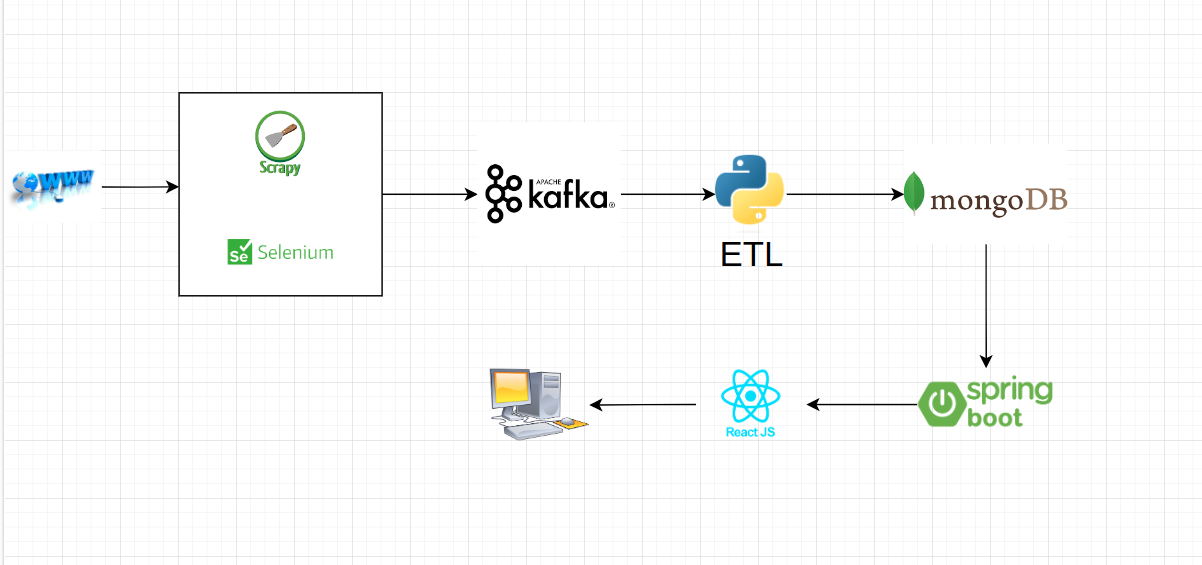
\includegraphics[scale=0.4]{Hinhve/architecture_system.png}
\begin{figure}[H]
    \centering
    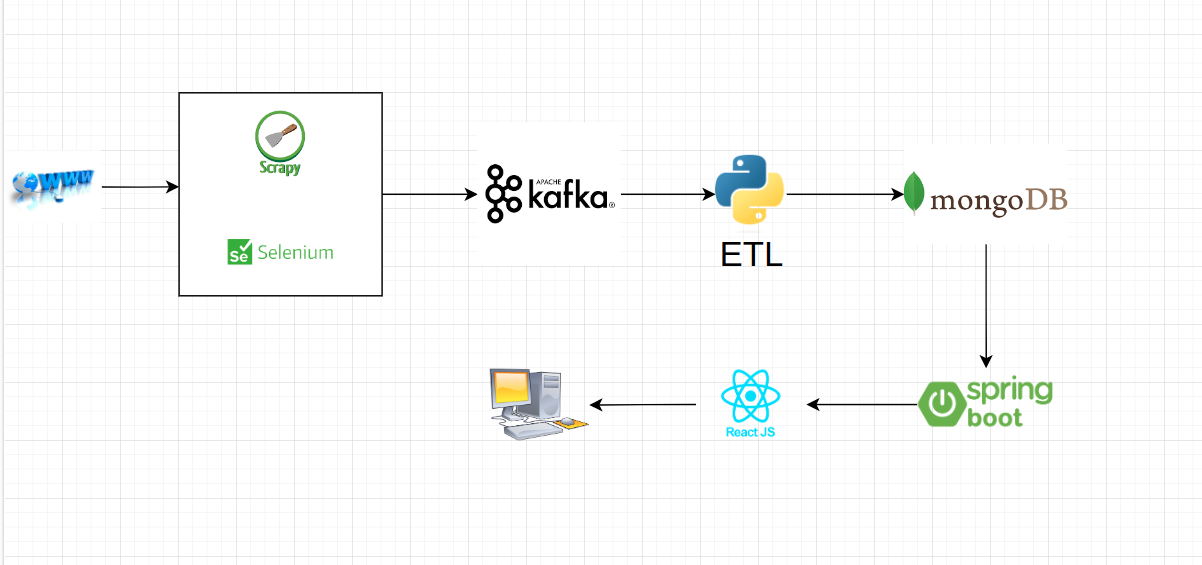
\includegraphics[scale=0.33]{Hinhve/architecture_system.png}
    \caption{Kiến trúc tổng quan của hệ thống}
    \label{fig:my_label2}
\end{figure}

Hệ thống được chia làm các pha khác nhau mỗi pha ứng với một quá trình xử lý dữ liệu riêng (hệ thống thu thập dữ liệu, hệ thống lưu trữ, xử lý và tích hợp dữ liệu, hệ thống tìm kiếm dữ liệu). Hệ thống thu thập dữ liệu từ các nguồn khác nhau sử dụng 2 công nghệ Scrapy và Selenium bóc tách dữ liệu trực tiếp từ các trang web cần thu thập. Dữ liệu sau khi được bóc tách được lưu trữ trực tiếp vào các topic tương ứng trong cụm hàng đợi Kafka. Cụm kafka có chức năng lưu trữ các message, xử lý và phân phối dữ liệu trực tiếp trong thời gian thực đồng thời đảm bảo độ tin cậy, độ trễ thấp và khả năng mở rộng cao. Sau khi dữ liệu được đẩy vào Kafka, hệ thống ETL sẽ lấy dữ liệu từ các topic đóng vai trò như consumer làm đầu vào cho quá trình làm sạch dữ liệu loại bỏ những kí tự đặc biệt, chuẩn hóa dữ liệu đưa về dạng thống nhất sau đó tiến hành tích hợp dữ liệu nhóm những sản phẩm lại với nhau nếu cùng là một loại theo định nghĩa. Dữ liệu sau khi được xử lý sẽ được lưu trữ tại cơ sở dữ liệu MongoDB Cloud - hệ quản trị cơ sở dư liệu phi quan hệ nằm trên đám mây. Hệ thống ứng dụng tìm kiếm sẽ truy vấn dữ liệu từ kho dữ liệu (datawarehouse) để phục vụ các chức năng của hệ thống tìm kiếm so sánh, phân tích thị trường ,...

\section{Hệ thống thu thập dữ liệu}
\subsection{Mô tả nguồn dữ liệu}
Nguồn dữ liệu của bài toán là những trang website trực tuyến uy tín chuyên cung cấp sản phẩm Apple chính hãng và dữ liệu cần thu thập ở đây là thông tin chi tiết về sản phẩm ví dụ như thông tin về thông số kĩ thuật, thông tin về giá cả thời điểm hiện tại, các đặc điểm ngoại hình màu sắc,... Trong hệ thống này em đang triển khai thu thập dữ liệu của khoảng 12 trang web được chia thành 2 loại dữ liệu chính: dữ liệu về thông tin chi tiết của sản phẩm còn lại là dữ liệu về thông giá cả và các thông tin liên quan.

% 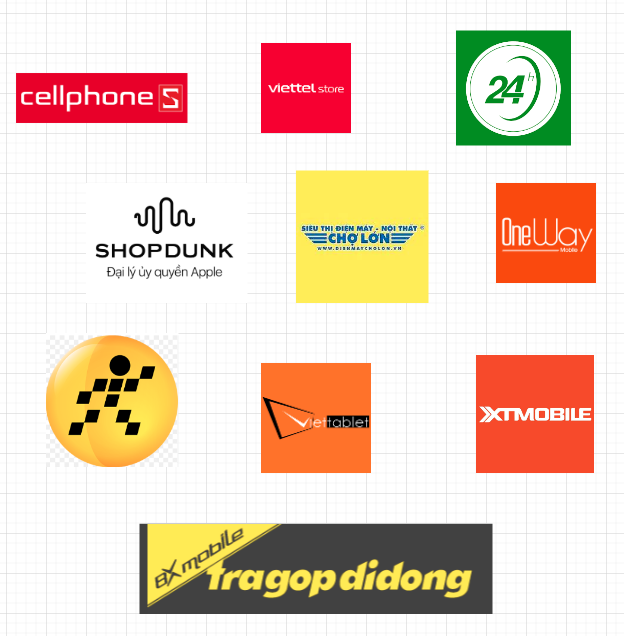
\includegraphics[scale=0.7]{Hinhve/data_sources.png}
\begin{figure}[H]
    \centering
    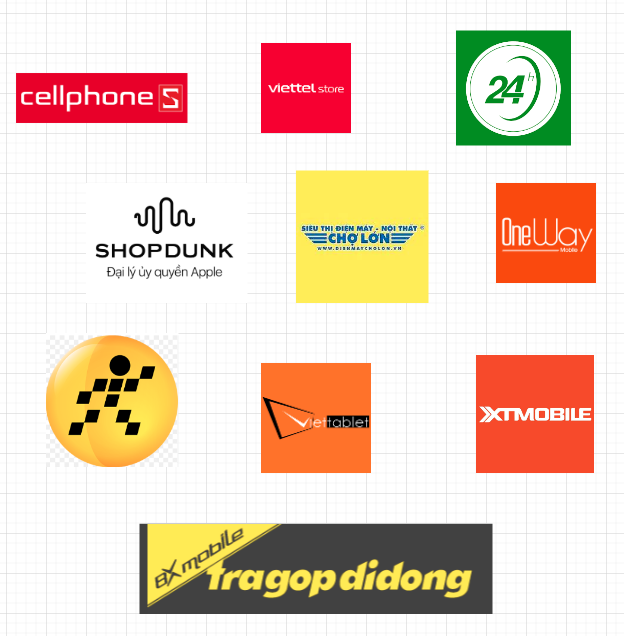
\includegraphics[scale=0.7]{Hinhve/data_sources.png}
    \caption{Nguồn dữ liệu thu thập}
    \label{fig:my_label2}
\end{figure}

Với từng trang web, hệ thống sẽ thu thập bóc tách trực tiếp sử dụng framework Scrapy (đối với trang web tĩnh) hoặc Selenium (đối với trang web động).Hệ thống đòi hỏi thu thập toàn bộ dữ liệu quan tâm hàng ngày, nhanh chóng, chính xác và việc mở rộng thêm các nguồn sau này một cách dễ dàng.

\subsection{Thu thập dữ liệu thông tin kĩ thuật}
\label{subsection:4.2.2.1}
Thu thập dữ liệu thông tin kĩ thuật của sản phẩm là quá trình thu thập dữ liệu từ một trang web chuyên cung cấp thông tin chi tiết về thông số cũng như bảo hành của các sản phẩm khác nhau đặc biệt là Apple. Bởi vì đây là hệ thống so sánh giá hàng ngày mà thông tin chi tiết về sản phẩm là không đổi nên việc thu thập dữ liệu toàn bộ thông tin về sản phẩm lặp lại là dư thừa và làm cho hệ thống trở nên chậm hơn, phát sinh nhiều lỗi không mong muốn. Để giảm thiểu tối đa rủi ro về hiệu năng cũng như tăng khả năng mở rộng nguồn dữ liệu nên em quyết định thu thập dữ liệu thông tin chi tiết độc lập và coi đây là một bảng dữ liệu thay đổi chậm (slow change) trong kiến trúc mô hình kho dữ liệu (data warehouse).

Quá trình thu thập dữ liệu sử dụng Python API của thư viện Selenium theo các bước sau:
\begin{itemize}
    \item Khởi tạo webdriver(Firefox) với các thông số cấu hình (headless,..), khởi tạo các url gốc là điểm xuất phát của chương trình thu thập:
    
    https://www.gsmarena.com/apple-phones-48.php,
    https://www.gsmarena.com/apple-phones-f-48-0-p2.php,
    https://www.gsmarena.com/apple-phones-f-48-0-p3.php
    \item Với mỗi url xuất phát, driver sẽ tìm các phần tử thẻ a bằng cách sử dụng XPATH để tìm kiếm và trích xuất ra các url con (thông qua thuộc tính href) là đường dẫn đến các sản phẩm cần trích xuất thông tin.
    \item Với mỗi url con, driver chuyển hướng và tiếp tục tìm kiếm thông tin. Ở đây driver sẽ thu thập toàn bộ dữ liệu bảng chưa thông tin chi tiết của sản phẩm và lưu trữ.
    \item Thực hiện cho tới khi quét hết các url con 
\end{itemize}
Dưới đây là dữ liệu mẫu khi bóc tách được từ hệ thống thu thập. Các sản phẩm khác nhau sẽ có số trường cụ thể là khác nhau (dữ liệu dạng phi quan hệ NoSQL) cuối cùng sẽ được lưu trữ tại collection ProductDetail trên MongoDB Cloud.

% 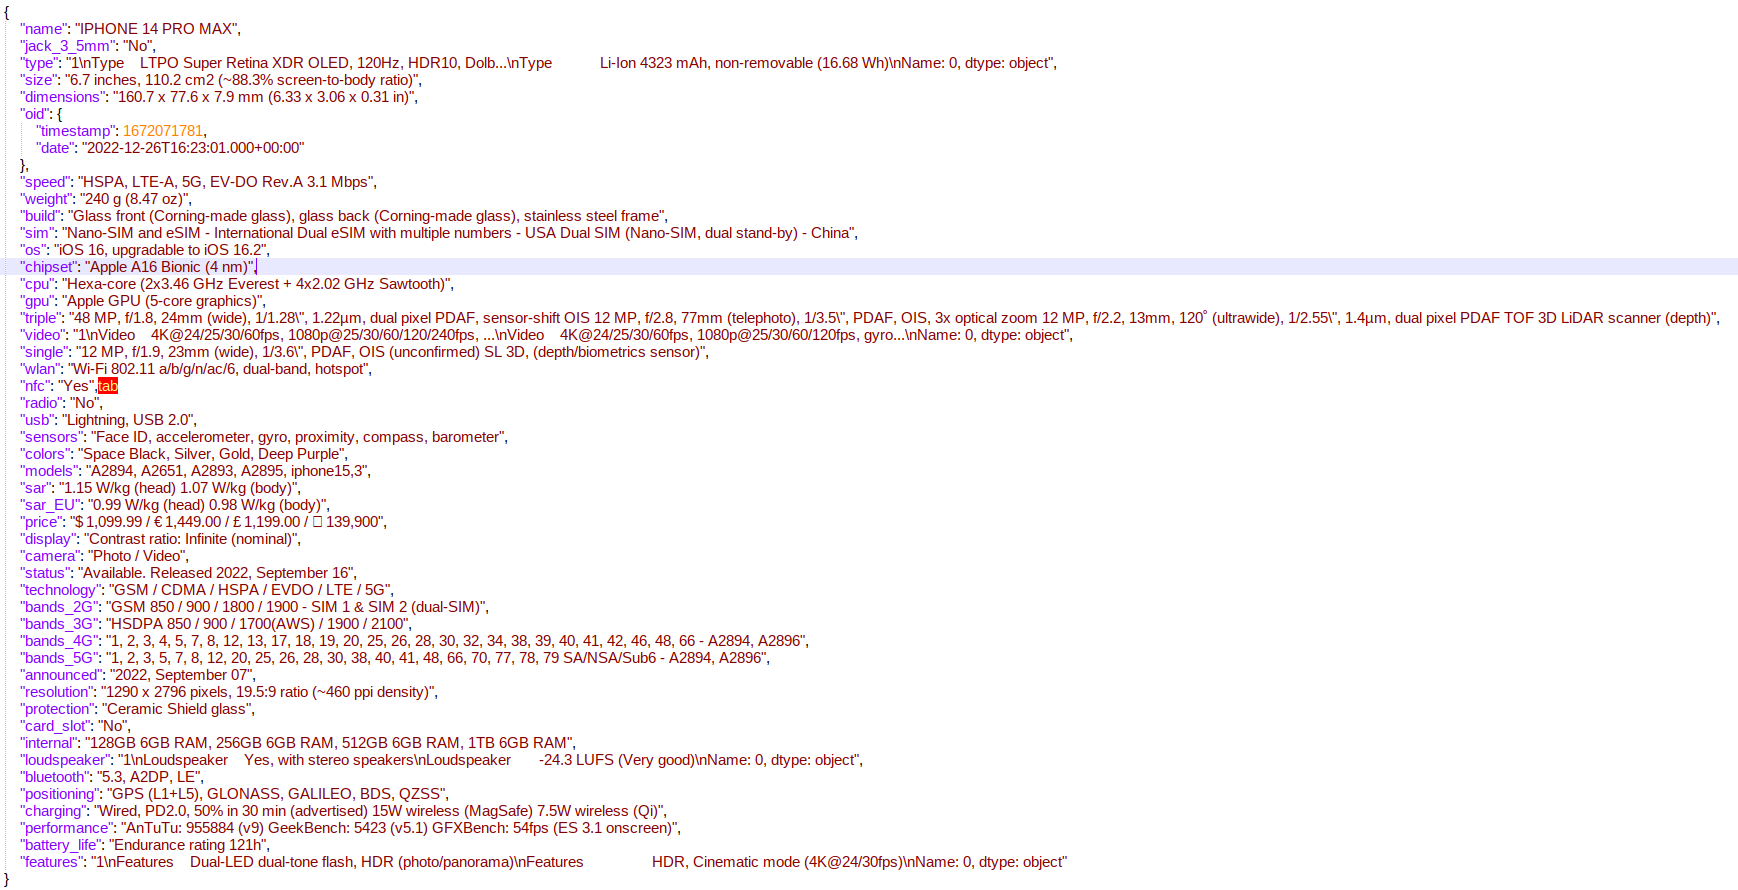
\includegraphics[scale=0.4]{Hinhve/info_product_example.png}
\begin{figure}[H]
    \centering
    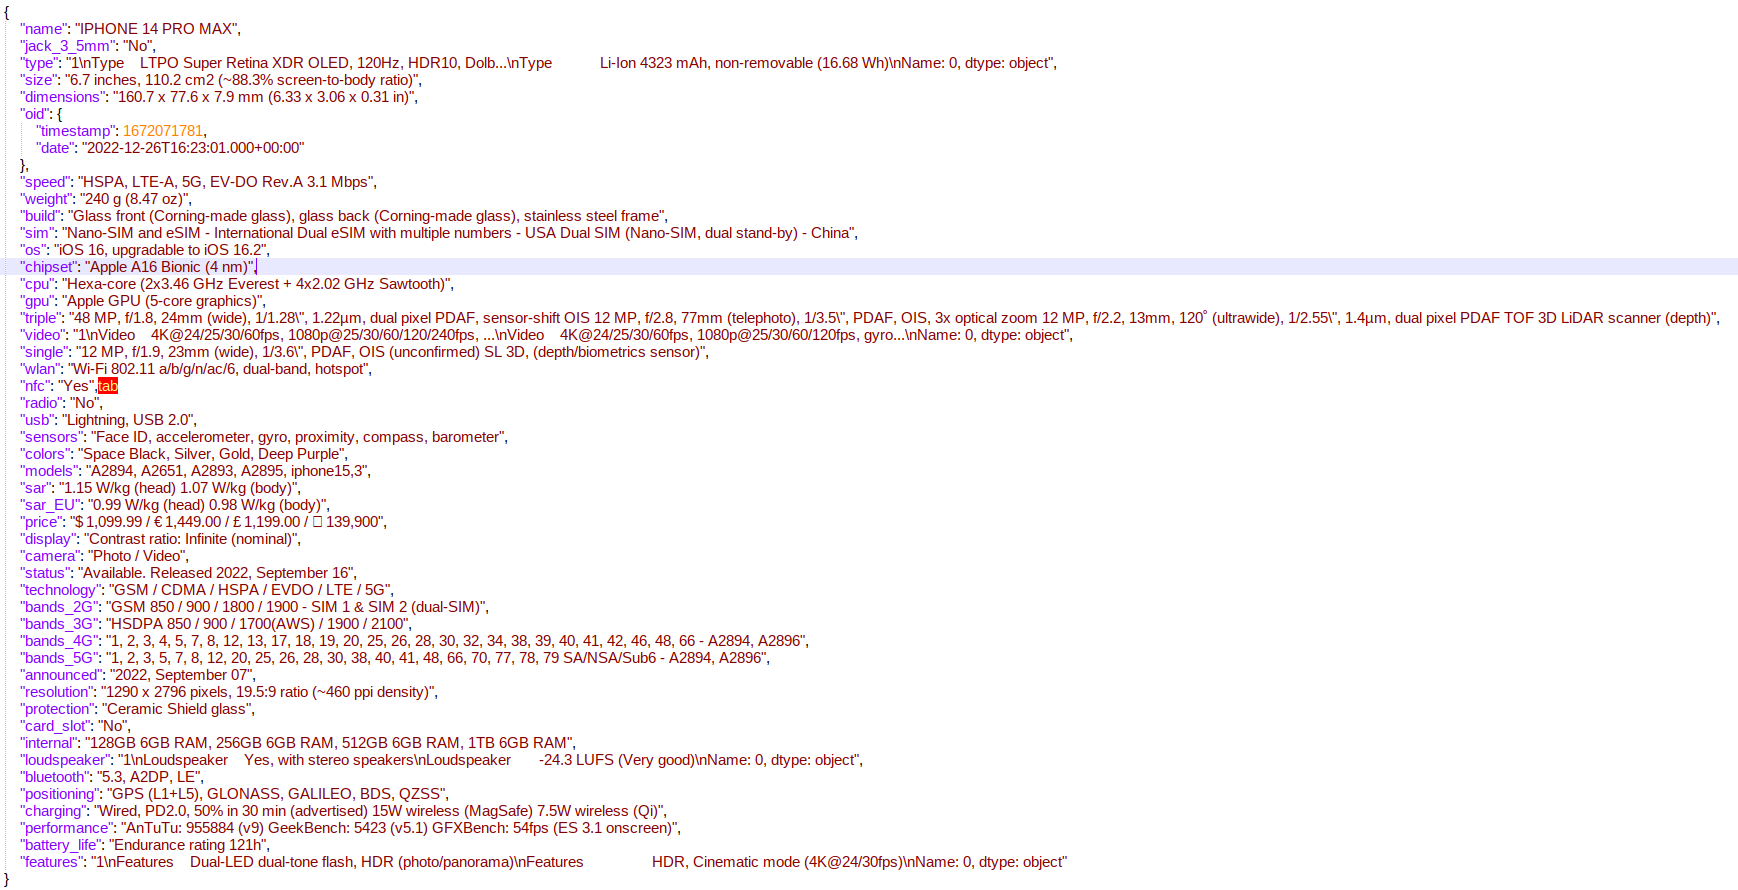
\includegraphics[scale=0.3]{Hinhve/info_product_example.png}
    \caption{Ví dụ bản ghi sản phẩm}
    \label{fig:my_label2}
\end{figure}

\subsection{Thu thập thông tin về giá cả}
\label{subsection:4.2.2.1}
Thông tin về giá cả được bóc tách trực tiếp từ các trang web được đề cập phía trên. Các trường thông tin mà hệ thống hướng đến để thu thập bao gồm thông tin về tên sản phẩm, màu sắc sản phẩm, dung lượng bộ nhớ trong, dung lượng bộ nhớ ngoài, đường dẫn tới sản phẩm, giá của sản phẩm,... Tùy vào từng nguồn dữ liệu, từng trang web mà số lượng trường dữ liệu có thể thay đổi bởi vì có một số trường hợp không bóc tách được do không tồn tại hoặc cú pháp phức tạp ảnh hưởng đến hiệu năng của hệ thống. 

Với mỗi trang web sẽ có quy trình, logic xử lý khác nhau tuy nhiên để mô tả tổng quát luồng xử lý thu thập dữ liệu em đã khái quát thông qua hình vẽ sau đây theo các bước xử  lý chung.

% 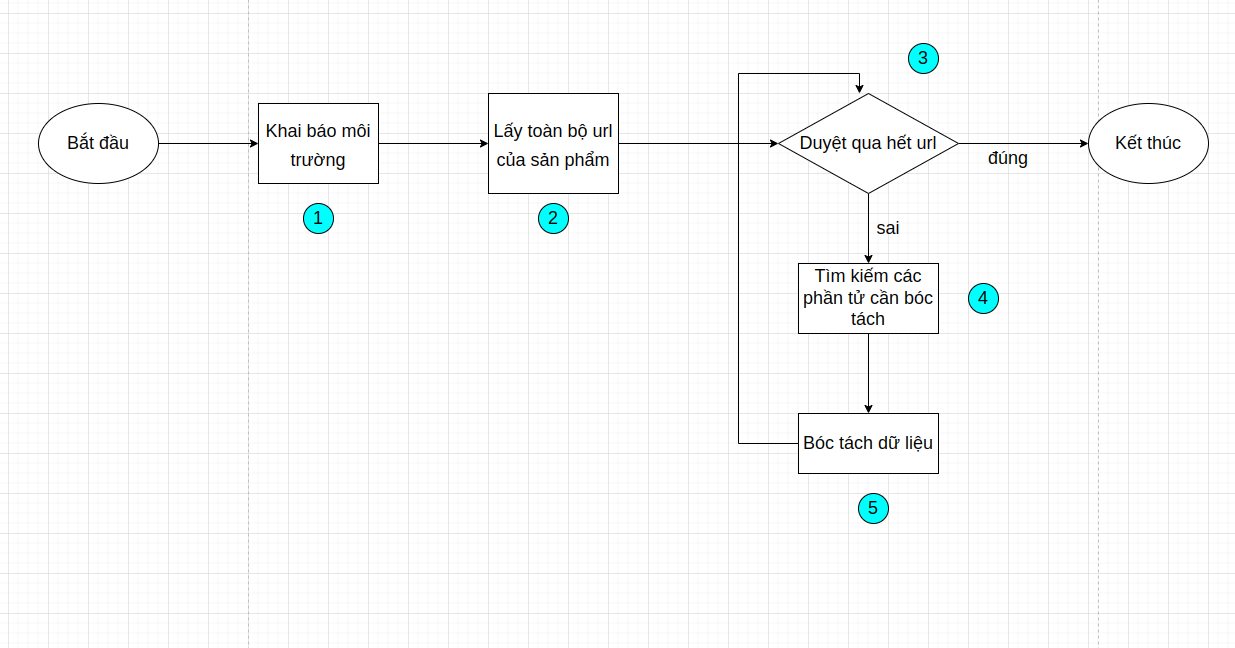
\includegraphics[scale=0.35]{Hinhve/overview_crawl.png}
\begin{figure}[H]
    \centering
    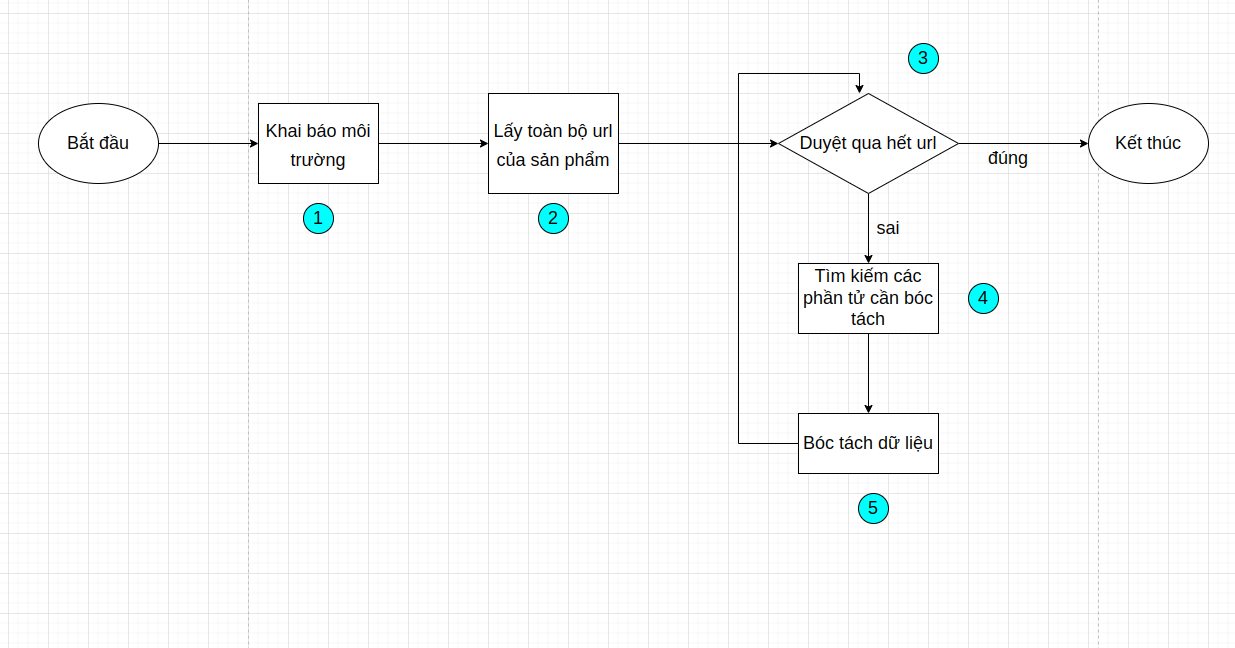
\includegraphics[scale=0.35]{Hinhve/overview_crawl.png}
    \caption{Tổng quan quá trình thu thâp dữ liệu}
    \label{fig:my_label2}
\end{figure}

\begin{itemize}
    \item Bước 1: Khai báo môi trường chung như ngày thu thập dữ liệu, kafka producer để lưu trữ dữ liệu thu thập được vào topic định nghĩa riêng đối với từng nguồn trong kafka. Ở bước này, chương trình có nhiệm vụ khai báo và tạo webdriver (đối với selenium), danh sách url gốc để thu thập dữ liệu, tên topic,... làm biến môi trường cho các bước sau.

    % 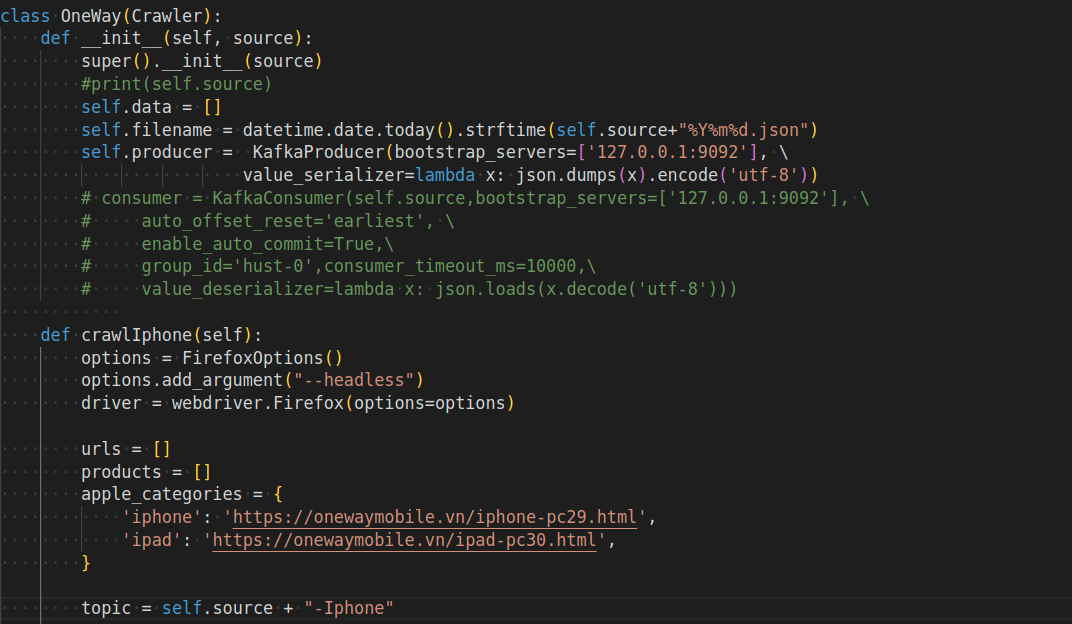
\includegraphics[scale=0.5]{Hinhve/step1_crawl_system.png}
    \begin{figure}[H]
        \centering
        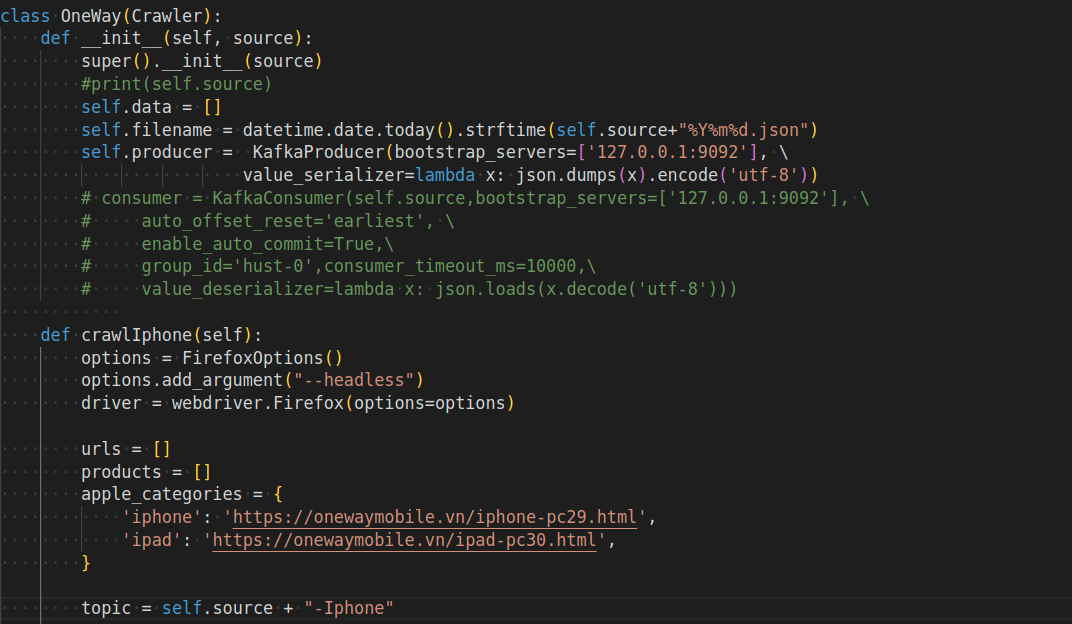
\includegraphics[scale=0.4]{Hinhve/step1_crawl_system.png}
        \caption{Bước 1 thu thập dữ liệu}
        \label{fig:my_label2}
    \end{figure}

    \item Bước 2: Lấy toàn bộ url của các sản phẩm trong trang web. Trường hợp 1 đối với các trang web không sử dụng javascript để sinh dữ liệu tại frontend công việc chỉ đơn giản là tìm các thẻ a trong HTML và trích xuất thuộc tính href bằng cách sử dụng XPATH để bóc tách. Trường hợp còn lại đối với các trang web sử dụng mã javascript để sinh dữ liệu (ví dụ xem thêm sản phẩm,...) thì có thêm một bước trung gian khác với mục đích tìm kiếm các button đó và thao tác để lấy được toàn bộ dữ liệu trang web (Selenium). 

    % 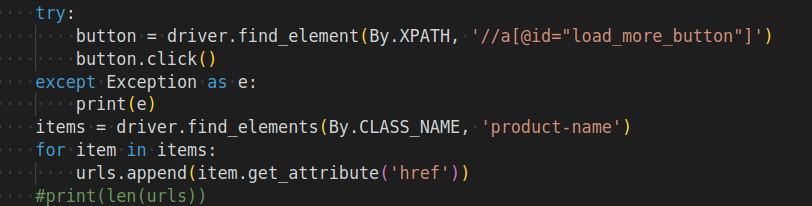
\includegraphics[scale=0.6]{Hinhve/step2_crawl_system.png}
    \begin{figure}[H]
        \centering
        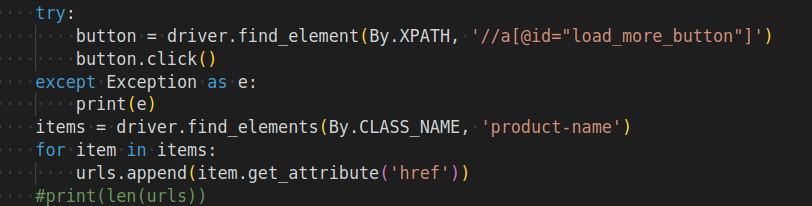
\includegraphics[scale=0.5]{Hinhve/step2_crawl_system.png}
        \caption{Bước 2 thu thập dữ liệu}
        \label{fig:my_label2}
    \end{figure}

    \item Bước 3: Bước điều kiện để kiểm tra đã duyệt qua tất cả url mà bóc tách bên trên chưa. Mỗi url ứng với một sản phẩm trong cửa hàng, mỗi sản phẩm có những thuộc tính khác nhau như màu sắc, bộ nhớ ngoài, bộ nhớ trong, trạng thái sản phẩm...

    \item Bước 4: Là bước quan trọng có nhiệm vụ bóc tách dữ liệu quan tâm (tên sản phẩm, màu sắc, giá cả, dung lương bộ nhớ trong, bộ nhớ ngoài, url, đường dẫn ảnh,...). Đối với mỗi nguồn dữ liệu, mỗi trang web lại có một cách bóc tách khác nhau tùy thuộc vào cấu trúc cũng như bố cục layout của trang web đó.

    % 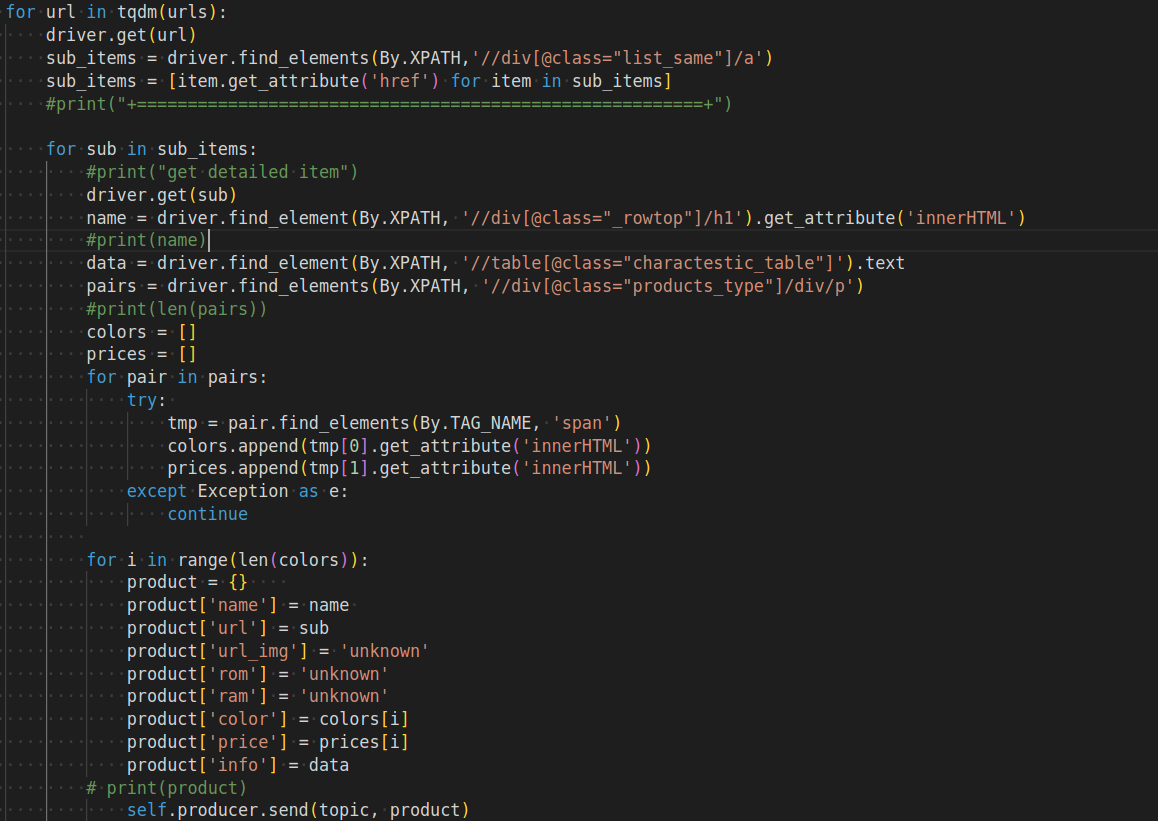
\includegraphics[scale=0.4]{Hinhve/step4_crawl_system.png}
    \begin{figure}[H]
        \centering
        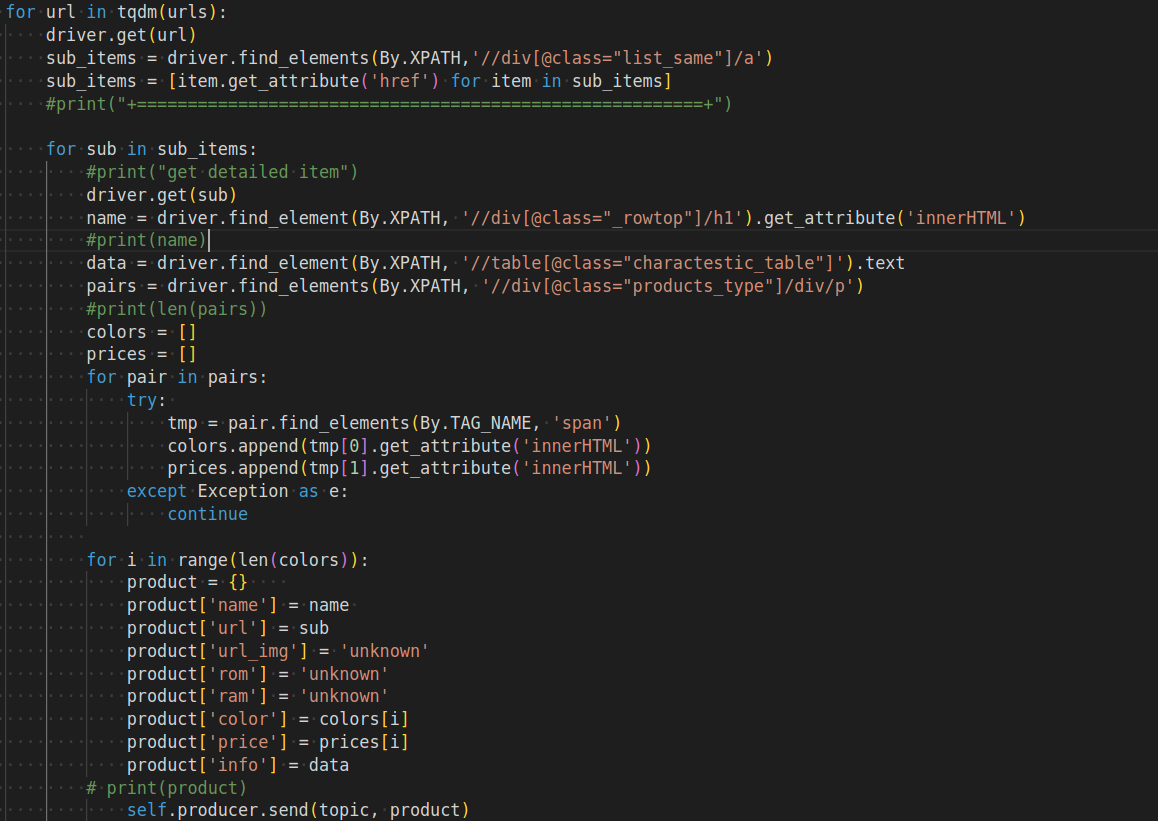
\includegraphics[scale=0.35]{Hinhve/step4_crawl_system.png}
        \caption{Bước 4 thu thập dữ liệu}
        \label{fig:my_label2}
    \end{figure}
    
    \item Bước 5: Là bước bóc tách các bản ghi dữ liệu và lưu trữ tại topic kafka đã được xác định tại bước 1.
\end{itemize}

Hệ thống thu thập dữ liệu được thiết kế độc lập, mỗi nguồn dữ liệu được xây dựng và cấu hình không phụ thuộc vào nhau. Do vậy luồng dữ liệu thu thập có thể chạy song song tùy thuộc vào phần cứng cũng như nhu cầu của người xây dựng luồng. Sau khi bóc tách kết thúc dữ liệu được lưu trữ tại kafka phục vụ cho các bước xử lý sau đó. 

\section{Hệ thống lưu trữ và xử lý dữ liệu}
\subsection{Ánh xạ lược đồ}
Bước đầu tiên trong hệ thống lưu trữ và xử lý dữ liệu là ánh xạ lược đồ  đảm bảo lược đồ  dữ liệu của các nguồn khác nhau được chuyển đổi về một lược đồ chung thống nhất theo tiêu chí số lượng các trường, kiểu dữ liệu cùng mô tả về một đặc tính duy nhất của dữ liệu (sản phẩm Apple). Để thực hiện điều đó em đã khảo sát và thực hiện và thiết kế  cấu trúc lược đồ chung cho toàn bộ dữ liệu bao gồm 9 trường thông tin khác nhau chủ yếu là các thông tin chính được thu thập từ các trang web mua bán trực tuyến.

\begin{itemize}
    \item name: Tên của sản phẩm tìm kiếm
    \item url: Đường dẫn tới nơi mà sản phẩm được bán
    \item ram: Bộ nhớ trong của sản phẩm
    \item rom: Bộ nhớ ngoài của sản phẩm
    \item price: Giá cả hiện tại của sản phẩm tại nơi bán
    \item createdDate: Ngày cập nhật 
    \item color: Màu sắc của sản phẩm
    \item status: Tình trạng hiện tại của sản phẩm (còn mới hay đã qua sử dụng)
    \item urlimg: Đường dẫn tới ảnh đại diện cho sản phẩm
\end{itemize}

Cách tiếp cận ở đây là hệ thống sẽ khai báo các consumer để  đọc dữ liệu liên tục từ các topic đã định nghĩa sẵn đối với từng nguồn dữ liệu trong kafka. Mỗi nguồn dữ liệu sẽ ứng với một luồng xử lý riêng biệt có thể thực hiện song song hóa cải thiện đáng kể hiệu năng của hệ thống. Sau khi đọc dữ liệu thô, các luồng xử lý đồng thời sẽ thực hiện ánh xạ lược đồ để biến đổi lược đồ gốc về lược đồ chung tổng quát của hệ thống kho dữ liệu. Phương pháp ánh xạ lược đồ ở đây em sẽ định nghĩa các luật ánh xạ đối với từng nguồn sau khi khảo sát các nguồn dữ liệu. Sau đó từ những luật đã định nghĩa thực hiện lần lượt trên các cột của lược đồ gốc ánh xạ tương ứng cuối cùng ta thu được một lược đồ chung.

% 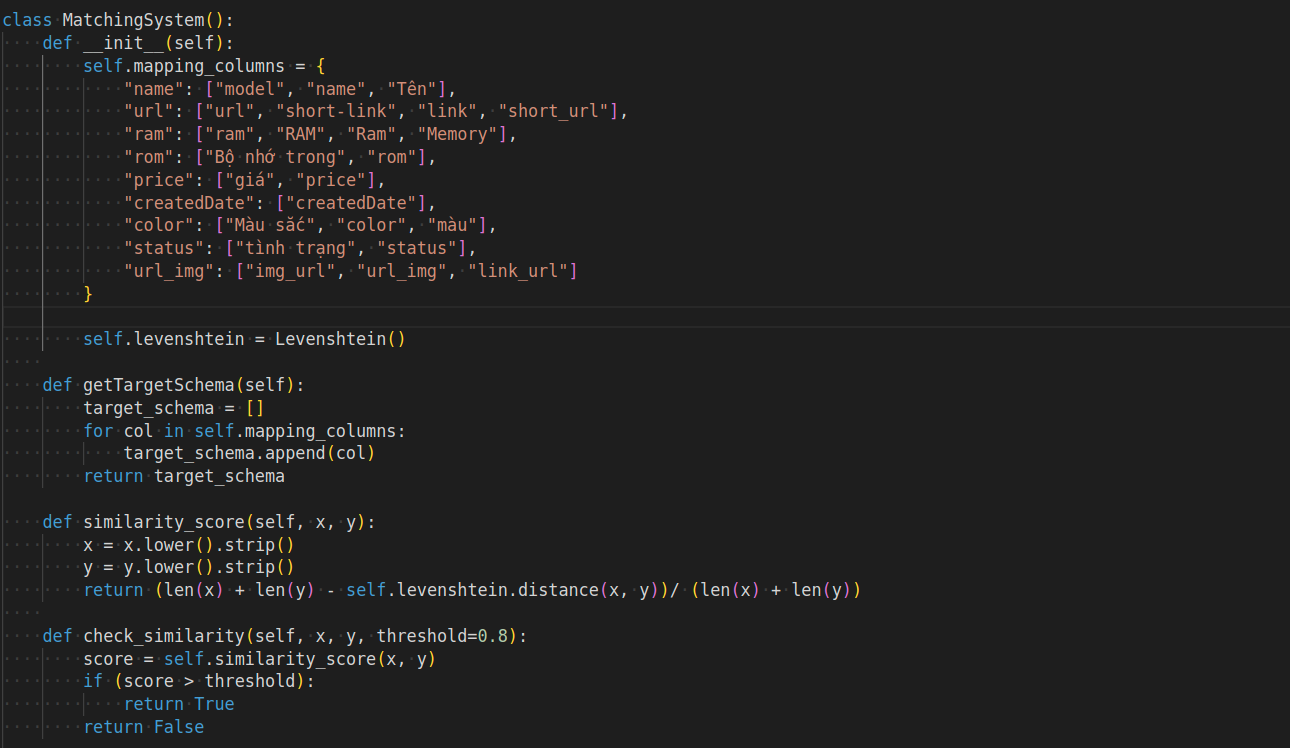
\includegraphics[scale=0.5]{Hinhve/schema_matching.png}
\begin{figure}[H]
    \centering
    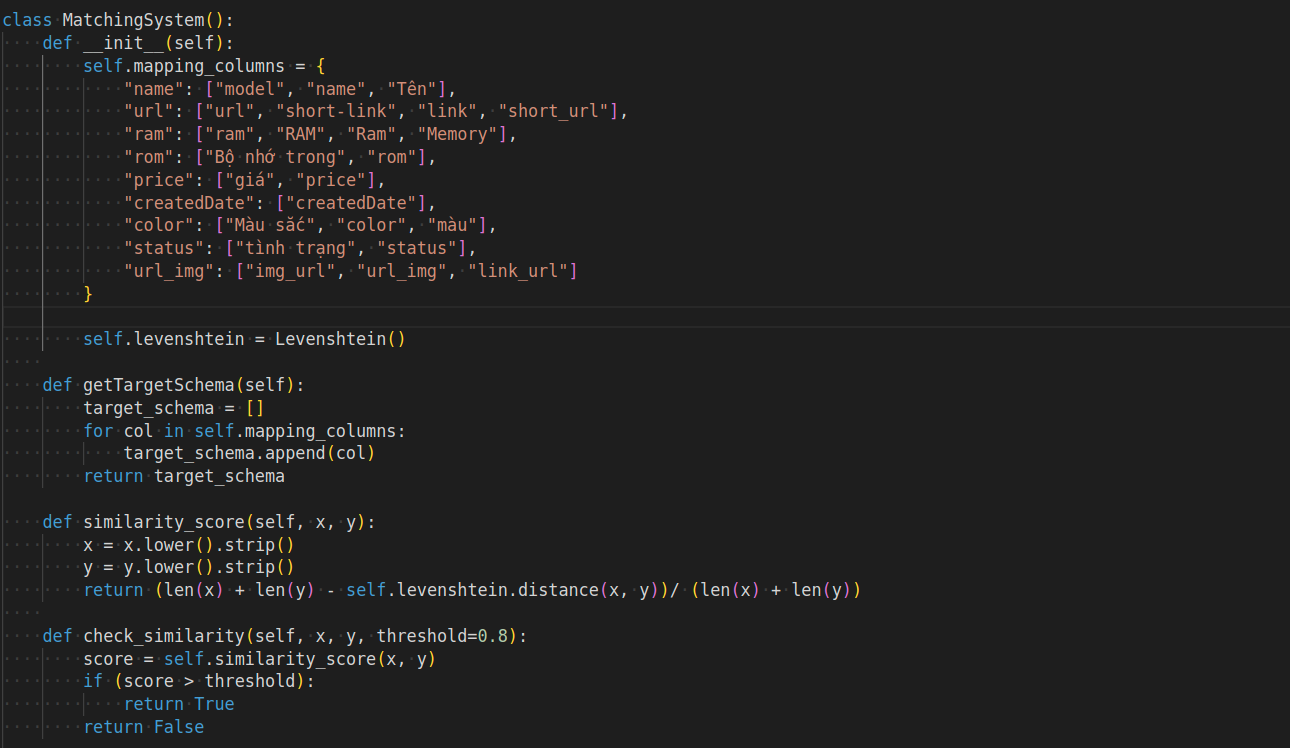
\includegraphics[scale=0.33]{Hinhve/schema_matching.png}
    \caption{Ánh xạ lược đồ}
    \label{fig:my_label2}
\end{figure}

Độ đo được sử dụng ở đây là độ đo tương đồng giữa hai chuỗi xâu dựa trên độ đo khoảng cách levenshtein được để cập ở chương trước với ngưỡng mặc định là 0,8. Ngưỡng này được chọn khi khảo sát và phân tích bản ghi tại các nguồn dữ liệu.Sau khi luồng xử lý kết thúc đầu ra của hệ thống sẽ là tập dữ liệu đã được đưa về lược đồ chung và làm đầu vào cho pha tiền xử lý dữ liệu ở bước sau.

\subsection{Tiền xử lý dữ liệu}
Tiền xử lý dữ liệu là quá trình chuẩn bị và xử lý dữ liệu trước khi chúng được sử dụng để xây dựng mô hình hoặc phân tích. Đây là một bước quan trọng trong quá trình khai phá dữ liệu, vì dữ liệu thường không được sạch sẽ và chuẩn hóa, và việc xử lý sai có thể dẫn đến các kết quả không chính xác. Sau bước ánh xạ lược đồ, luồng xử lý tiếp theo là tiền xử lý dữ liệu cho đầu ra của pha trước đó. Tại đây hệ thống tập trung chủ yếu xử lý các trường dữ liệu quan trọng có liên quan tới bước tích hợp dữ liệu đặc biệt là tên sản phẩm, màu sắc, ram, rom,.. với mục đích chuẩn hóa dữ liệu phục vụ cho quá trình so khớp dữ liệu. Sau đây là các bước tiền xử lý dữ liệu cơ bản:

\begin{itemize}
    \item Bước 1: Xử lý các giá trị bất thường. Dữ liệu thường bao gồm các giá trị bất thường. Điều này có thể dẫn đến các kết quả không chính xác khi phân tích dữ liệu. Hệ thống có thể xử lý các giá trị bất thường bằng cách loại bỏ chúng hoặc thay thế chúng bằng giá trị khác, chẳng hạn như giá trị trung bình. Tại đây hệ thống sẽ loại bỏ khoảng trắng ở hai đầu của chuỗi, những kí tự đặc biệt,... Bên cạnh đó lọc ra tất cả các bản ghi trùng lặp vì dữ liệu có thể lặp lại do việc thu thập hoặc đường dẫn liên kết đến sản phẩm trùng lặp. Bên cạnh đó hệ thống loại bỏ các bản ghi không phải sản phẩm của Apple, các bản ghi nhiễu thông tin của các trang web,... 

    % 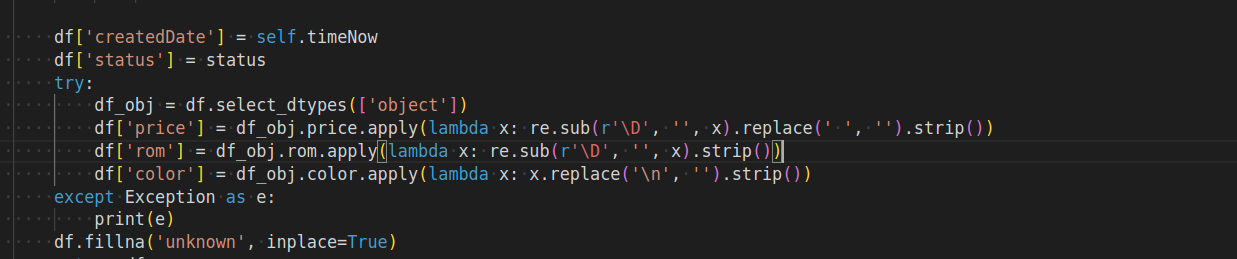
\includegraphics[scale=0.4]{Hinhve/preprocess_step1.png}
    \begin{figure}[H]
        \centering
        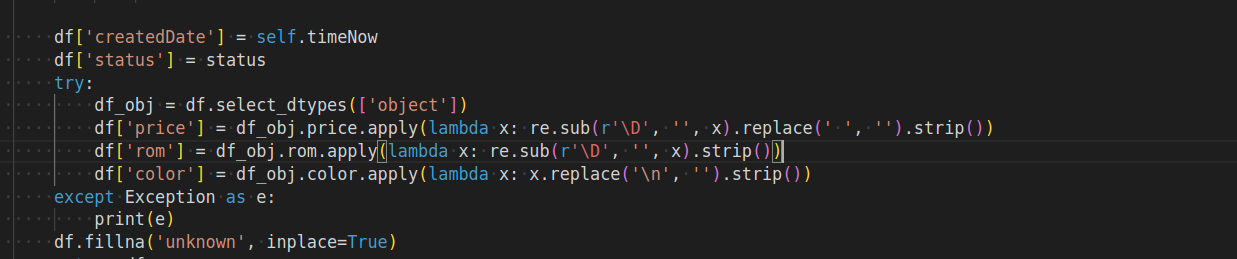
\includegraphics[scale=0.34]{Hinhve/preprocess_step1.png}
        \caption{Tiền xử lý bước 1}
        \label{fig:my_label2}
    \end{figure}
    Một số trường hợp đặc biệt khi thu thập dữ liệu một số bản ghi chứa nhiều thông tin của các trường khác nhau như trường tên thông tin sản phẩm thường chứa các thông tin khác như màu sắc, dung lượng bộ nhớ trong, dung lượng bộ nhớ ngoài,... Hệ thống xử lý trích xuất các trường này giúp cho tập dữ liệu đầy đủ, chính xác. Một trường hợp khác dữ liệu có thể chứa một danh sách các giá trị của một thuộc tính, nhiệm vụ của hệ thống sẽ trích xúât các giá trị đó và phân tách thành các bản ghi khác nhau làm giàu dữ liệu cho kho dữ liệu.

    % 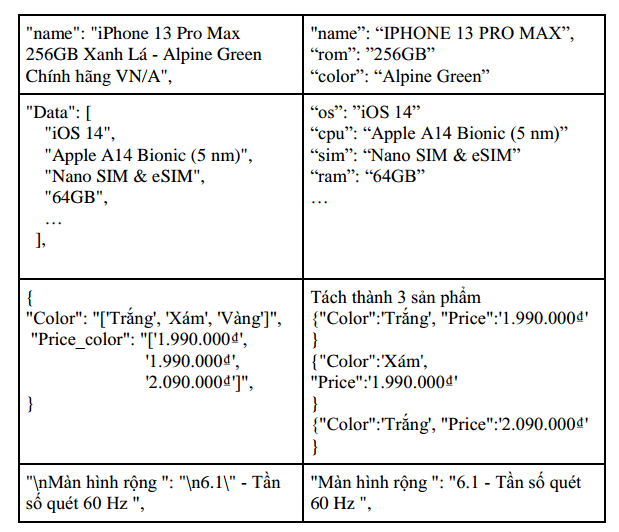
\includegraphics[scale=0.5]{Hinhve/preprocess_step1_res.png}
    \begin{figure}[H]
        \centering
        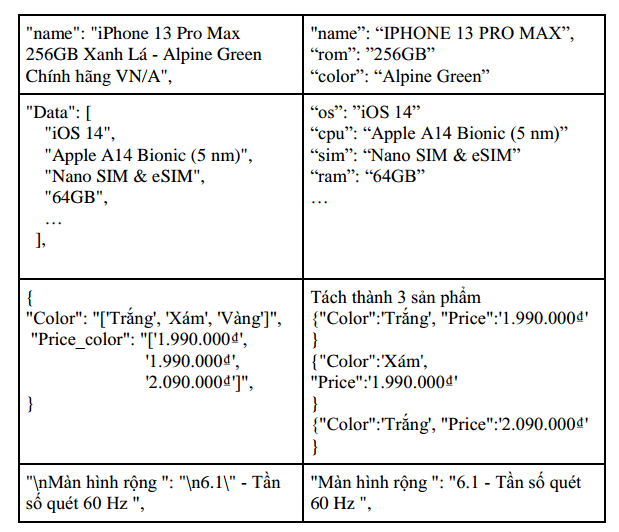
\includegraphics[scale=0.62]{Hinhve/preprocess_step1_res.png}
        \caption{Kết quả tiền xử lý bước 1}
        \label{fig:my_label2}
    \end{figure}
    \item Bước 2: Chuẩn hóa dữ liệu về định dạng chung. Dữ liệu thường được lưu trữ dưới nhiều dạng khác nhau và đơn vị đo lường khác nhau. Tại đây hệ thống chuyển đổi dữ liệu về cùng một đơn vị đo lường và định dạng để phù hợp với mô hình hoặc phân tích. Đối với dữ liệu số loại bỏ các kí tự không phải số và ép kiểu về giá trị số thực như giá của sản phẩm, dung lượng bộ nhớ trong, dung lượng bố nhớ ngoài,... Bước này đóng vai trò rất quan trọng ảnh hưởng trực tiếp tới pha tiếp theo của hệ thống. Hệ thống tập trung xử lý chặt chẽ trường thông tin liên quan tới tên sản phẩm bởi vì nó có trọng số lớn trong mô hình tích hợp dữ liệu để cho ra thông tin đạt độ chính xác cao. Bên cạnh đó một số trường thông tin cũng rất quan trọng như giá sản phẩm, thông tin vê sản phẩm cũng được xử lý. Phương pháp tiếp cận chủ yếu ở bước này là sử dụng một tập hợp các ánh xạ tên sản phẩm được định nghĩa sẵn như sau:

    % 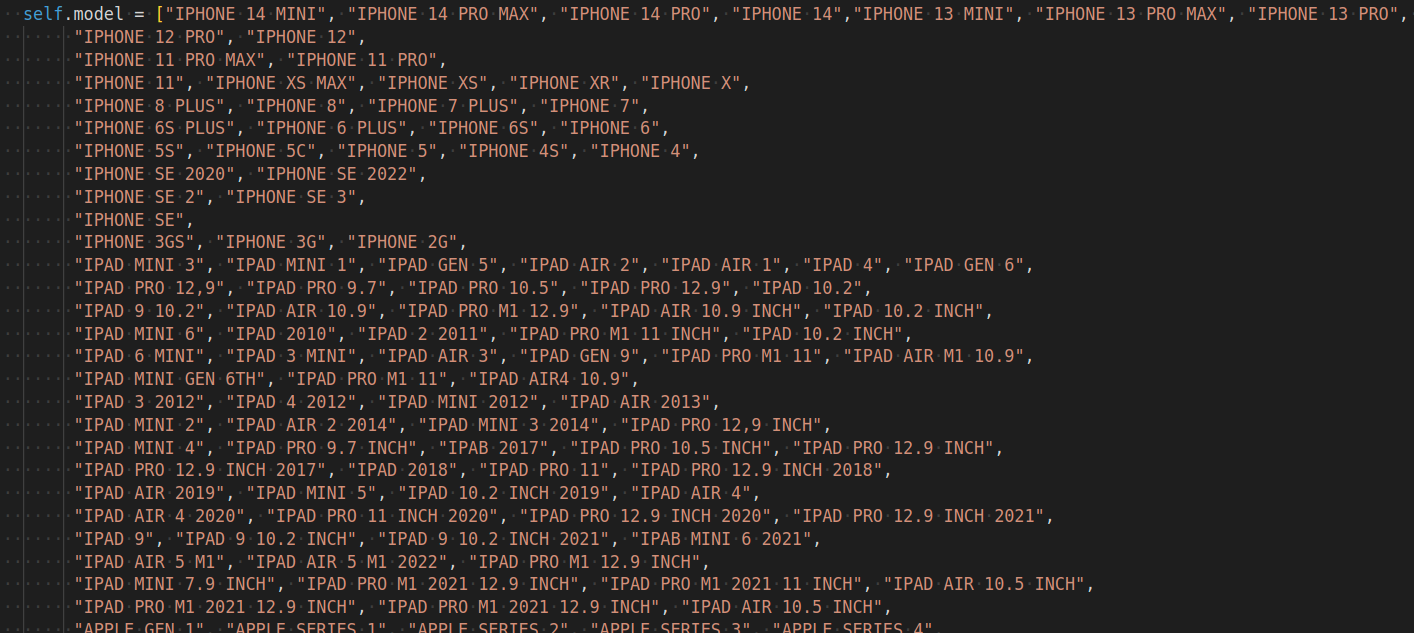
\includegraphics[scale=0.4]{Hinhve/preprocess_step2.png}

    \begin{figure}[H]
        \centering
        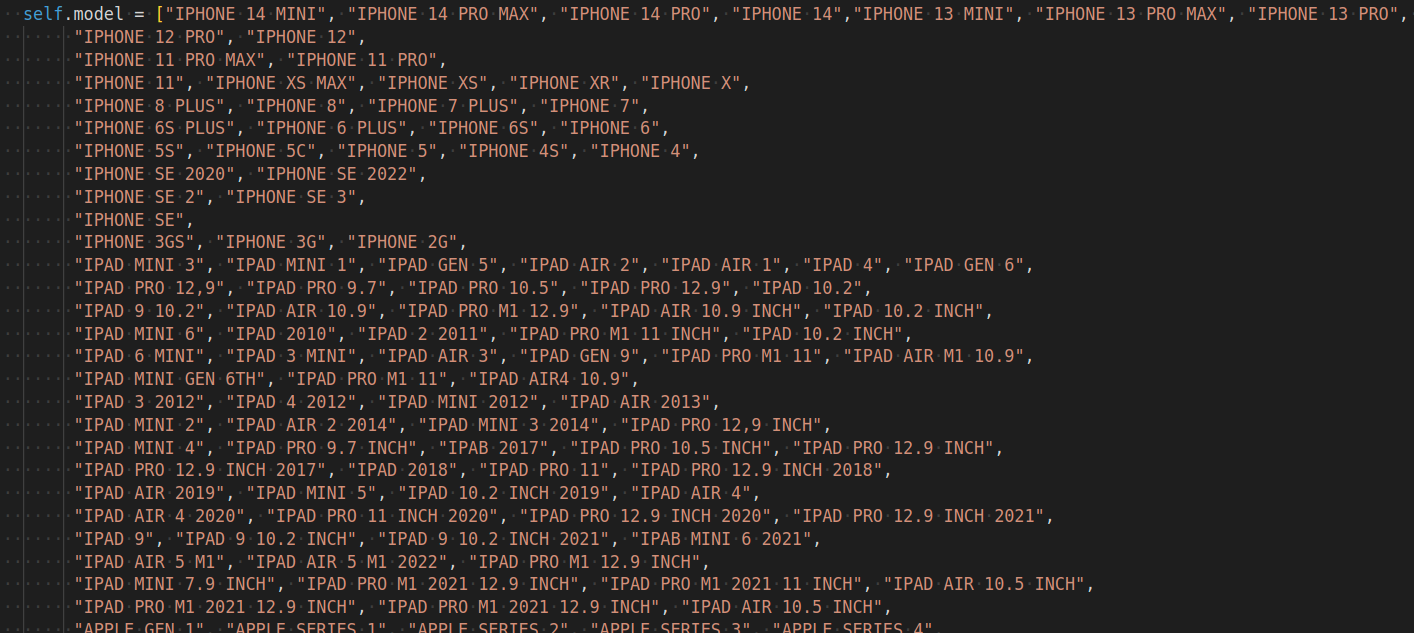
\includegraphics[scale=0.3]{Hinhve/preprocess_step2.png}
        \caption{Tiền xử lý bước 2}
        \label{fig:my_label2}
    \end{figure}

    Hệ thống duyệt lần lượt qua các bản ghi chuẩn hóa theo tên sản phẩm đã được định nghĩa đối với trường thông tin tên bên cạnh đó chuẩn hóa giá, màu sắc, rom, ram về cùng một định dạng chung.Sau khi tiền xử lý xong, dữ liệu của hệ thống có dạng như sau
\end{itemize}

% 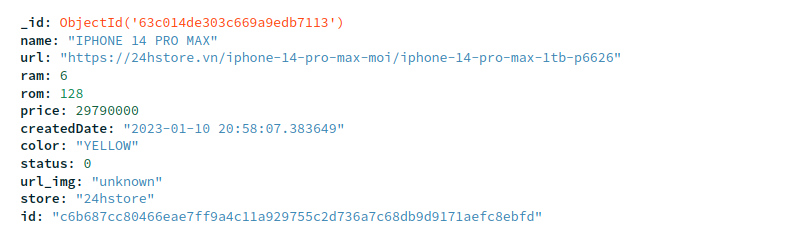
\includegraphics[scale=0.7]{Hinhve/preprocess_final_res.png}
\begin{figure}[H]
    \centering
    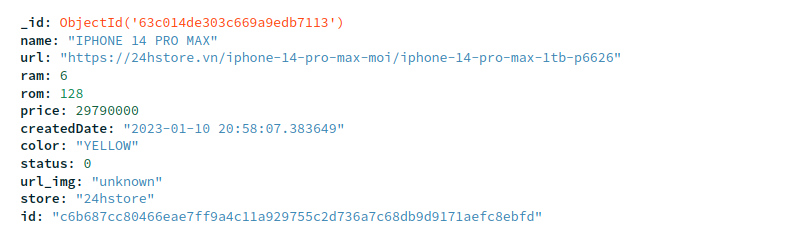
\includegraphics[scale=0.68]{Hinhve/preprocess_final_res.png}
    \caption{Kết quả tiền xử lý dữ liệu}
    \label{fig:my_label2}
\end{figure}

\subsection{Tích hợp dữ liệu}
Tích hợp dữ liệu hay so khớp dữ liệu là quá trình phân cụm dữ liệu chia một tập hợp thành các nhóm sản phẩm khác nhau. Mỗi một nhóm sản phẩm đề cập tới một loại sản phẩm mà người dùng định nghĩa. Trong bài toán này một sản phẩm đươc định nghĩa phân biệt bởi các trường sau: tên sản phẩm, màu sắc của sản phẩm, dung lượng bộ nhớ trong, dung lượng bộ nhớ ngoài, trạng thái của sản phẩm (cũ hay mới). Mục tiêu cuối cùng của pha này là phân cụm toàn bộ sản phẩm thành các cụm dữ liệu sao cho số lượng cụm tương đương với loại sản phẩm định nghĩa trên. 

Phương pháp đối sánh dữ liệu ở đây sử dụng phương pháp đánh trọng số cho các thuộc tính (name, ram, rom, color, status) trong đó việc so khớp tên của hai xâu sử dụng độ đo khoảng cách chỉnh sửa và chuẩn hóa về khoảng 0 và 1. Bên cạnh đó hệ thống cũng dựa trên độ đo khác biệt tự định nghĩa. Các trường có giá trị "unknown" của một sản phẩm sẽ luôn khớp với trường đó của sản phẩm khác bởi vì dữ liệu thường chưa đầy đủ. Hệ thống sẽ duyệt lần lượt các sản phẩm và đối sánh với nhau để tính ra độ tương đồng của sản phẩm nếu hai sản phẩm có độ tương đồng lớn hơn một ngưỡng nhất định thì hai sản phẩm đó cùng thuộc một cụm sản phẩm ngựợc lại hai sản phẩm ở hai cụm sản phẩm khác nhau dưới đây là công thức tính độ đo tương đồng.

Bên cạnh đó để phân biệt từng sản phẩm theo định nghĩa của người dùng, hệ thống có sử dụng hàm băm sha-256 để sinh ra khóa phân biệt chúng. SHA256 là một thuật toán mã hóa băm (hashing algorithm) mà sử dụng để tạo ra một giá trị băm (hash value) duy nhất cho dữ liệu đầu vào. Thuật toán này có thể được sử dụng để đảm bảo tính toàn vẹn của dữ liệu hoặc để bảo mật thông tin. SHA256 là viết tắt của "Secure Hash Algorithm 256-bit", và nó sử dụng một khối đầu vào dữ liệu với kích thước tối đa là 
$2^{64})$ bit để tạo ra một giá trị băm dài 256-bit. Kết quả đầu ra của SHA256 là một chuỗi 256-bit (32-byte) duy nhất, được biểu diễn dưới dạng chuỗi ký tự hexa. SHA256 là một trong những thuật toán băm phổ biến và được sử dụng rộng rãi trong các ứng dụng bảo mật, chẳng hạn như chứng thực thông tin hay xác thực người dùng. 

% 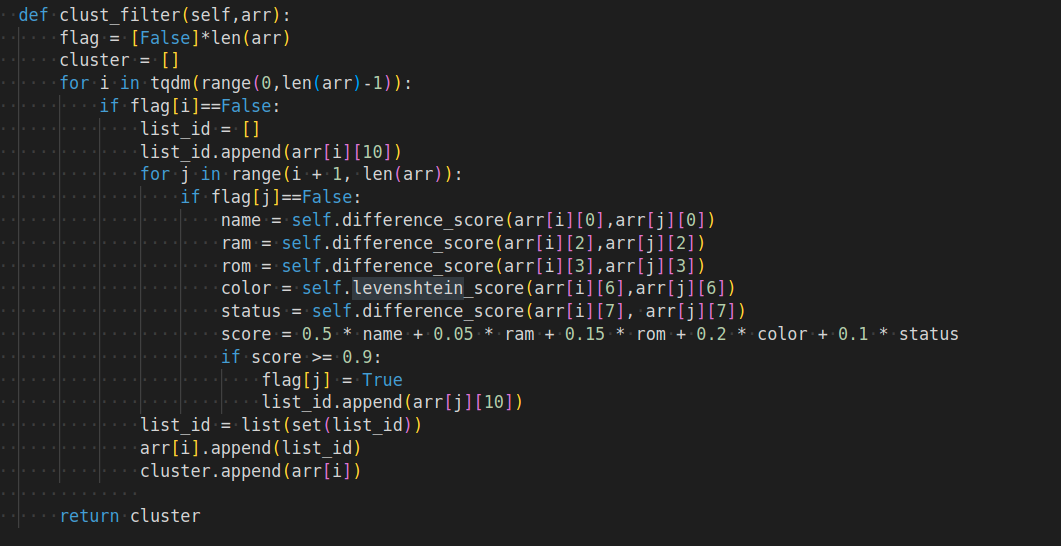
\includegraphics[scale=0.5]{Hinhve/data_matching.png}
\begin{figure}[H]
    \centering
    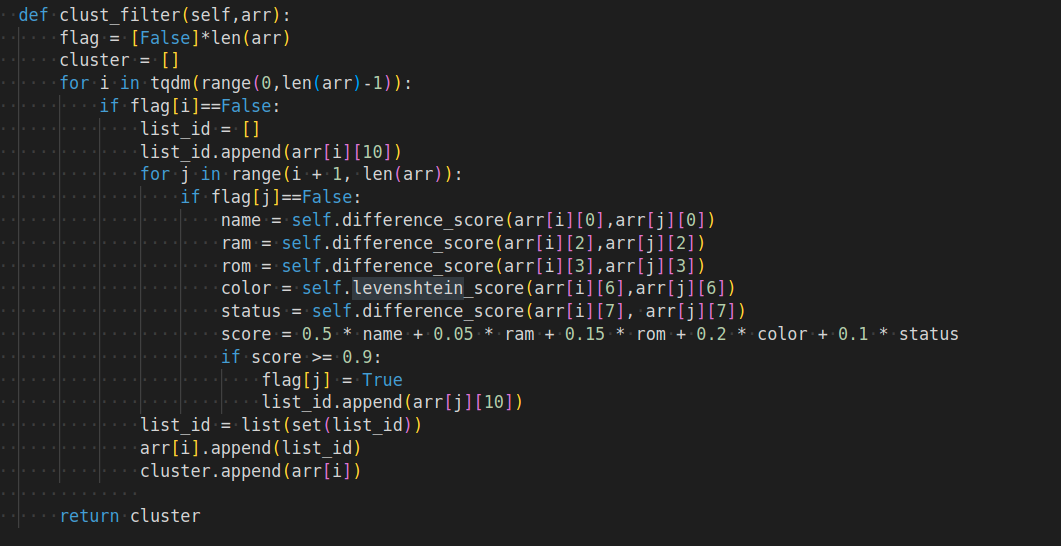
\includegraphics[scale=0.42]{Hinhve/data_matching.png}
    \caption{So khớp dữ liệu}
    \label{fig:my_label2}
\end{figure}

Hệ thống so khớp duyệt qua toàn bộ dữ liệu và kết quả cuối cùng tạo thành các cụm sản phẩm. Kết quả phân cụm được lưu trữ tại một bảng được đồng bộ và sử dụng như bảng tìm kiếm sản phẩm tầng ứng dụng. Đối với một bản ghi dữ liệu mới được thêm vào hệ thống, nếu bản ghi này đã tồn tại trong hệ thống cơ sở dữ liệu sẽ tự động cập nhật giá trị còn ngược lại nếu bản ghi không tồn tại, bộ so khớp sẽ tính toán độ tương đồng của điêm dữ liệu này so với các cụm để phân loại vào cụm thích hợp. Sau đây là một vài ví dụ về kết quả của các cụm sản phẩm

 % 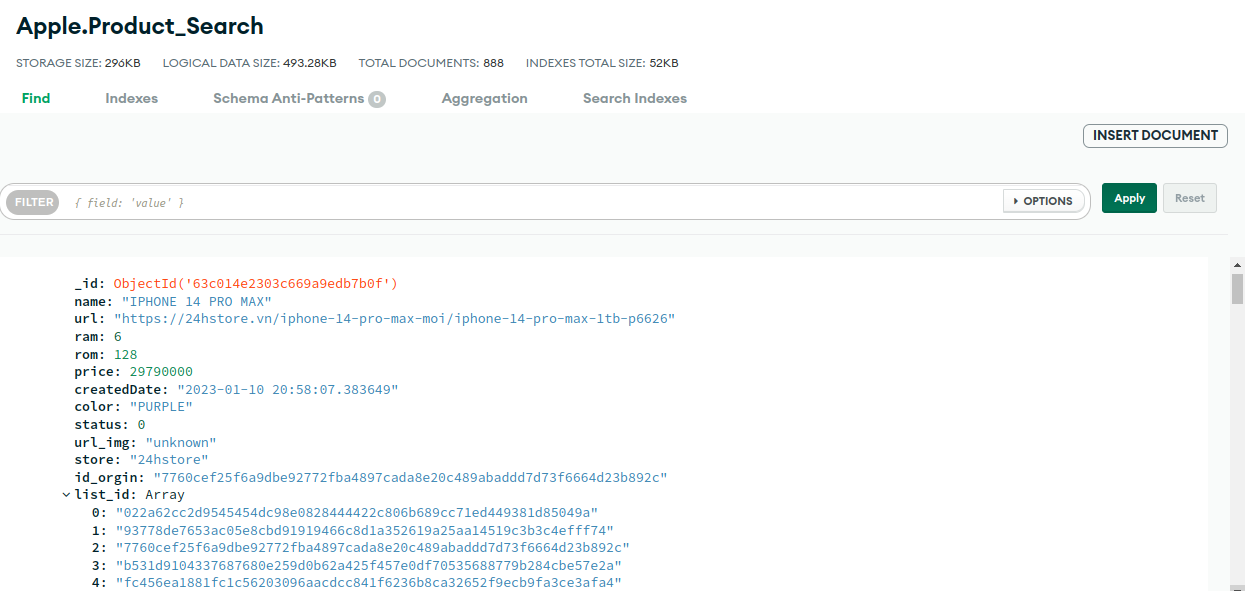
\includegraphics[scale=0.5]{Hinhve/data_matching_res.png}
 \begin{figure}[H]
    \centering
    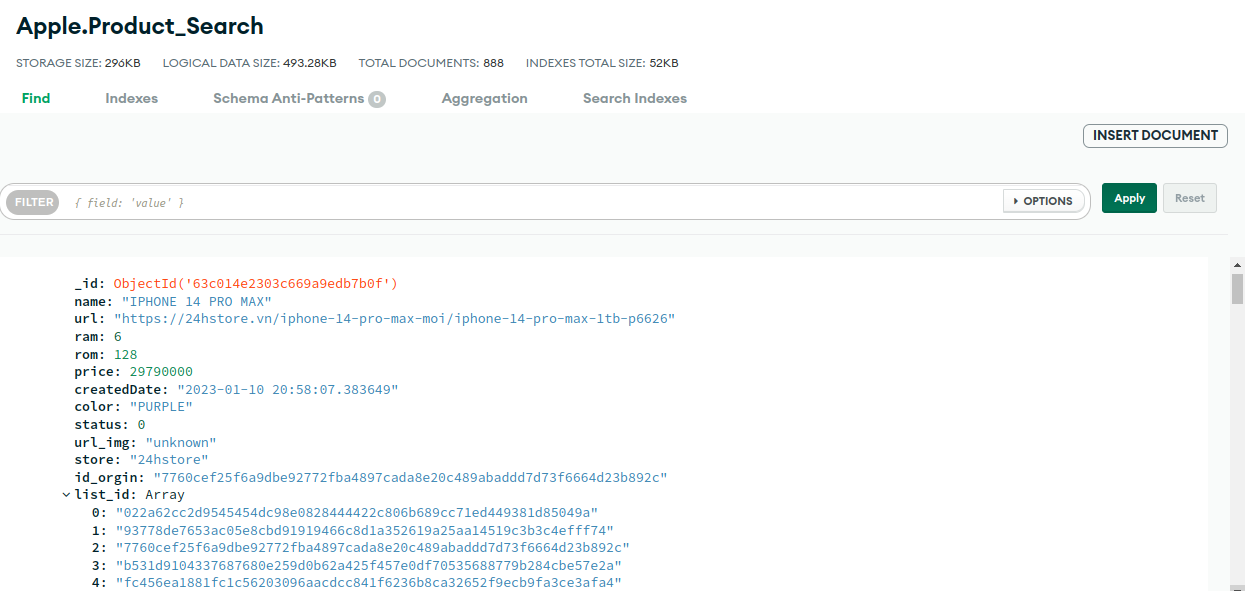
\includegraphics[scale=0.5]{Hinhve/data_matching_res.png}
    \caption{Kết quả so khớp dữ liệu}
    \label{fig:my_label2}
\end{figure}

 Sau khi so khớp dữ liệu được hoàn thành, hệ thống sẽ tự động cập nhật cũng như tải dữ liệu lên MongoDB cloud (hệ thống lưu trữ đám mây) lần lượt là các bảng 
 \begin{itemize}
     \item Products: Bảng chứa thông tin các sản phẩm của hệ thống
     \item ProductSearch: Bảng chứa thông tin tìm kiếm sản phẩm
     \item ProductDetail: Bảng chứa thông tin chi tiết về sản phẩm phục vụ việc tra cứu thông tin.
 \end{itemize}

 

Hệ thống tích hợp dữ liệu yêu cầu luồng dữ liệu được cập nhật hàng ngày đảm bảo dữ liệu luôn trong trạng thái sẵn sàng, mới nhất và kịp thời tới người dùng những người đang có nhu cầu mua sản phẩm phù hợp với họ. Để đáp ứng điều này mà không phải chạy thủ công, cần xây dựng một hệ thống lập lịch tự động chạy luồng hàng ngày để thu thập xử lý dữ liệu. Trong đồ án này em sử dụng crontab để lập lịch cho hệ thống tích hợp dữ liệu.

Crontab là một công cụ trong hệ thống Linux và Unix, cho phép người dùng lên lịch để thực hiện các tác vụ định kỳ hoặc lặp lại trong hệ thống. Crontab hoạt động dựa trên các tệp cấu hình được lưu trữ trên hệ thống, cho phép người dùng chỉ định các lệnh hoặc tập lệnh để thực hiện, và các điều kiện để xác định thời điểm cụ thể khi lệnh được thực thi. Với crontab, người dùng có thể lên lịch để thực hiện các tác vụ định kỳ như sao lưu dữ liệu, chạy các tác vụ định kỳ của hệ thống, định kỳ tạo bản ghi log, hoặc cập nhật các ứng dụng tự động. Crontab cũng cung cấp cho người dùng tính linh hoạt và tùy chỉnh cao, cho phép lên lịch thực hiện các tác vụ theo các kịch bản tùy chỉnh. Người quản trị thực hiện lập lịch chạy 5 giờ sáng hàng ngày để thu thập và tích hợp dữ liệu lên kho dữ liệu. Tùy thuộc vào cấu hình của phần cứng máy chủ mà có thể chạy song song nhiều tác vụ crontab khác nhau.Sau khi dữ liệu đã sẵn sàng, hệ thống tìm kiếm có thể truy vấn bảng để tìm kiếm những kết quả khớp với câu truy vấn đầu vào mà người dùng nhập. 
 
\section{Hệ thống ứng dụng tìm kiếm so sánh giá}
Hệ thống ứng dụng tìm kiêm so sánh giá là một trang web đơn giản giúp người dùng có thể tìm kiếm sản phẩm với việc nhập thông tin các trường tên sản phẩm, màu sắc, dung lượng bộ nhớ trong, dung lượng bộ nhớ ngoài,... Như đã giới thiệu ở chương 3, hệ thống tìm kiếm sử dụng reactJs để xây dựng giao diện chính cho trang web. Chi tiết cách xây dựng cũng như vẽ các giao diện được trình bày chi tiết trong mã nguồn của hệ thống. Sau đây là một vài kết quả chính mà hệ thống ứng dụng có thể cung cấp cho người dùng

\begin{figure}[H]
    \centering
    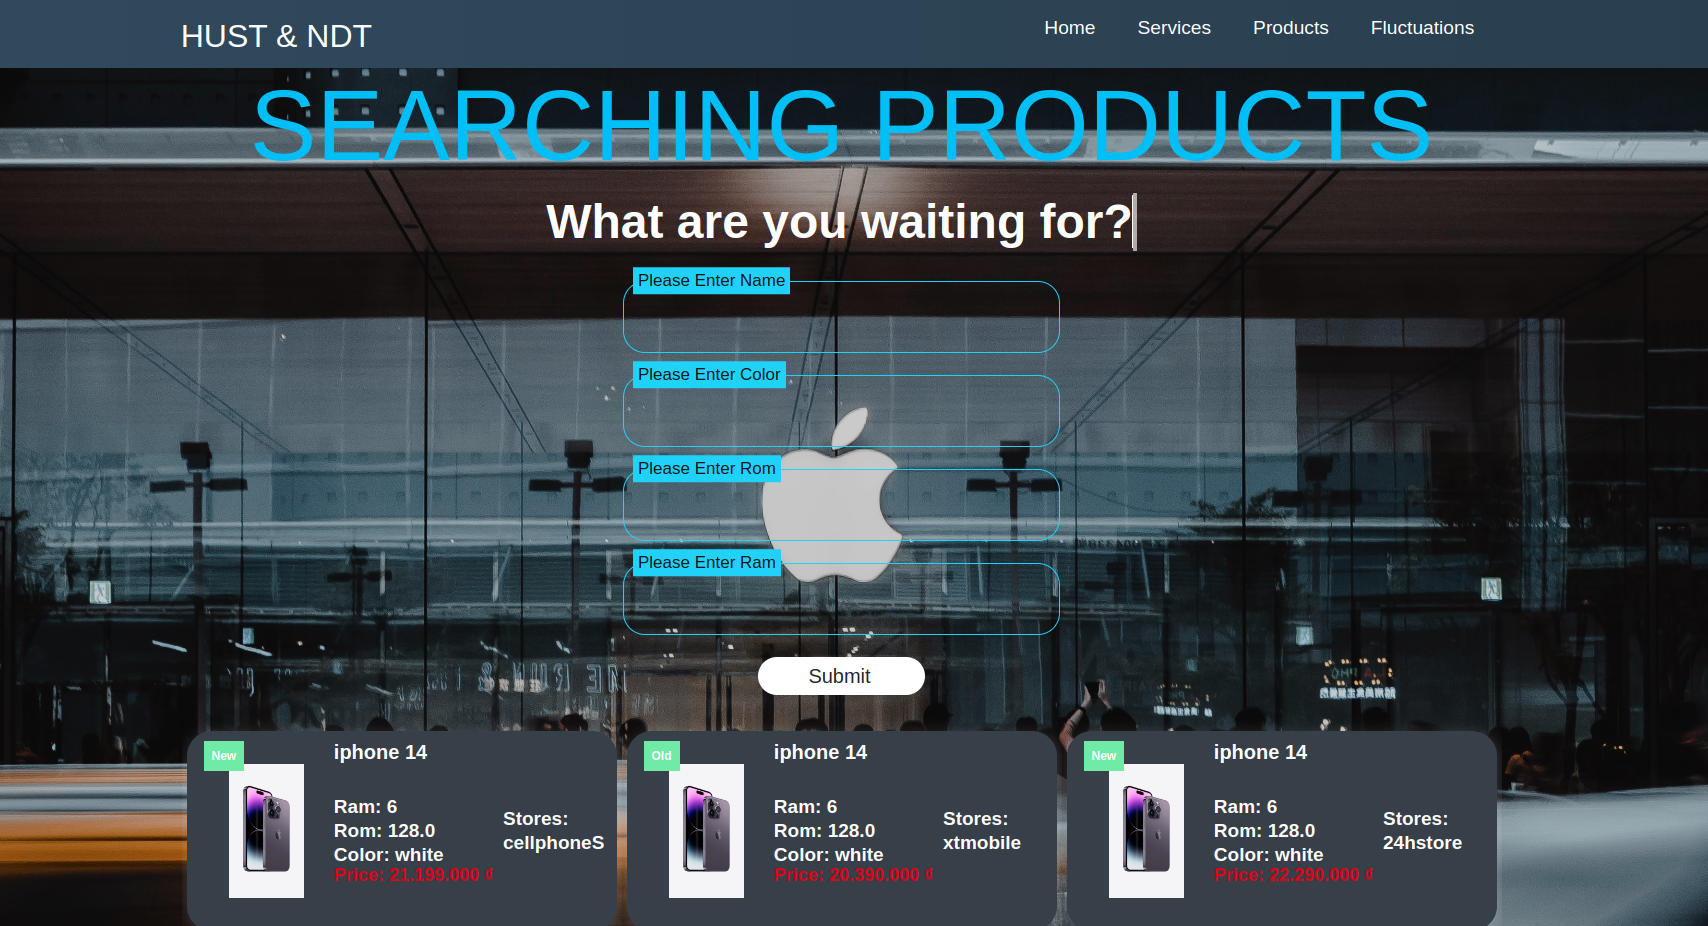
\includegraphics[scale=0.25]{Hinhve/searchUI_01.png}
    \caption{Màn hình tìm kiếm}
    \label{fig:my_label}
\end{figure}

Sau khi nhập thông tin cần tìm kiếm người dùng nhấn vào button tìm kiếm hệ thống sẽ tự động thực hiện câu lệnh truy vấn tới cơ sở dữ liệu để lấy ra một danh sách các kết quả và hiển thị trên màn hình. Người dùng sẽ tham khảo và chọn một trong các kết quả là sản phẩm quan tâm ứng với một danh sách các cửa hàng có bán sản phẩm đó sẽ được hiển thị trên màn hình.

\begin{figure}[H]
    \centering
    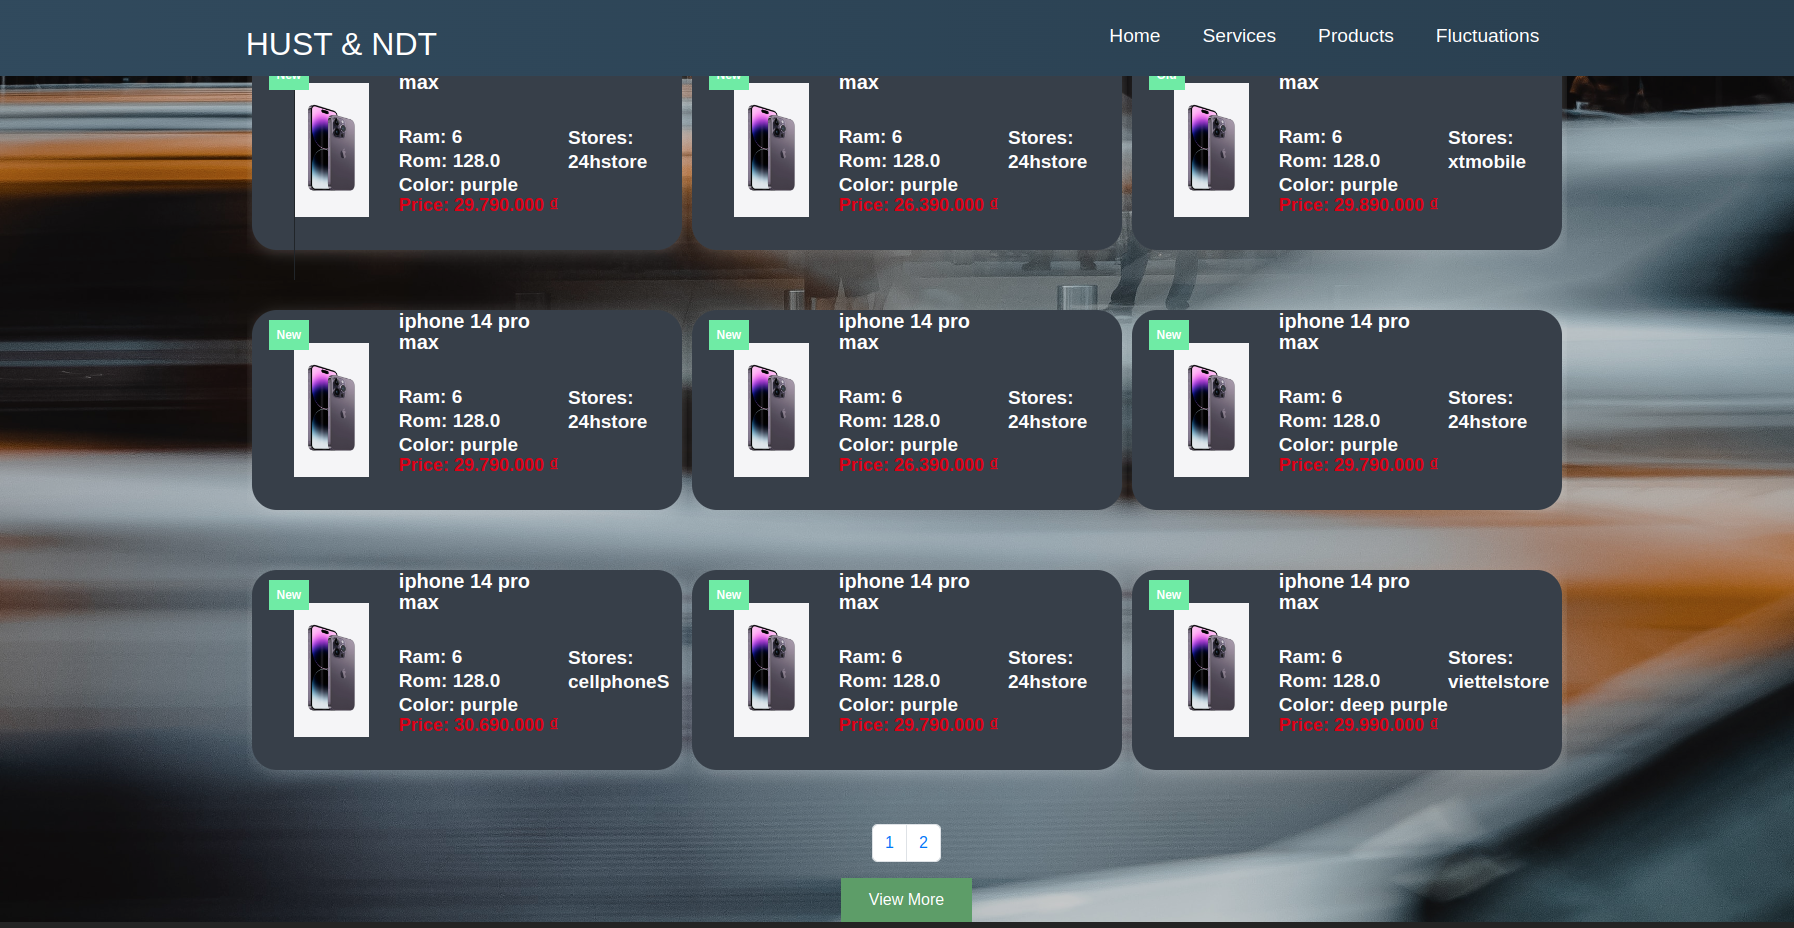
\includegraphics[scale=0.24]{Hinhve/searchUI_2.png}
    \caption{Màn hình kết quả}
    \label{fig:my_label2}
\end{figure}

Danh sách kết quả tìm kiếm sản phẩm được bán tại các cửa hàng được hiện thị trên màn hình. Người dùng chọn một thẻ kết quả, hệ thống tự động điều hướng tới nơi bán giúp cho việc tra cứu cũng như mua bán trở nên dễ dàng hơn. Bên cạnh đó,  người sử dụng có thể tra cứu và xem thông tin chi tiết của một sản phẩm về tất cả thông số kĩ thuật.

\begin{figure}[H]
    \centering
    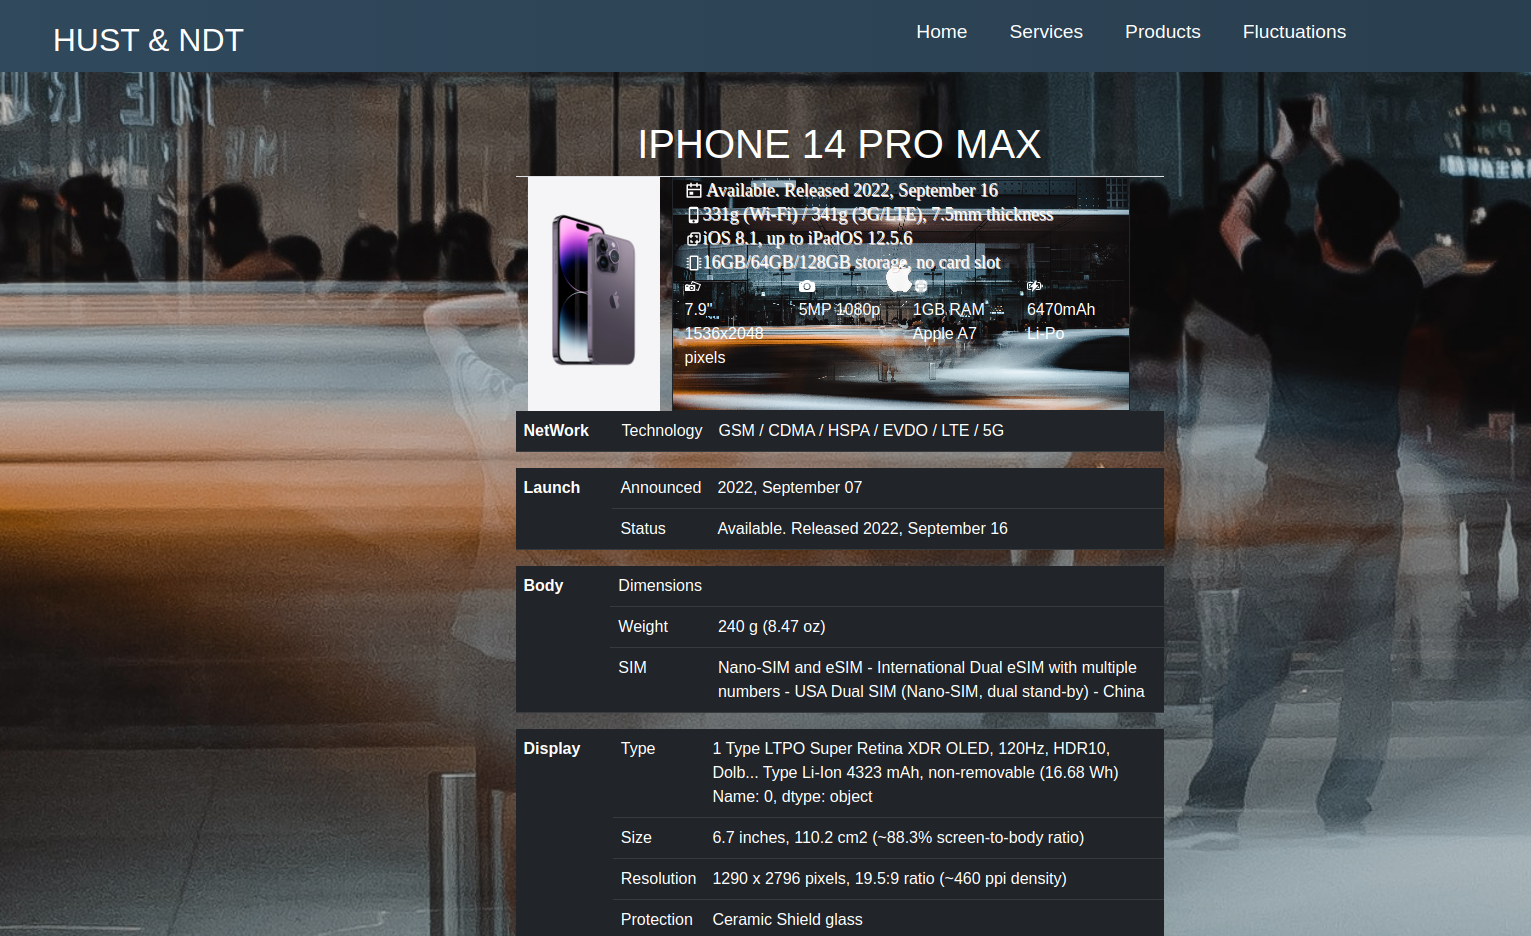
\includegraphics[scale=0.28]{Hinhve/info_UI.png}
    \caption{Màn hình thông tin sản phẩm}
    \label{fig:my_label2}
\end{figure}

Ngoài ra, người dùng có thể thống kê, xem các biểu đồ phân tích về thị trường sản phẩm được tích hợp trong hệ thống. Các biểu đồ này được định nghĩa và truy vấn dữ liệu trực tiếp từ MongoDB Cloud nên có thể dễ dàng thêm mới, sửa đổi hoặc xóa biểu đồ sao cho phù hợp với nhu cầu tra cứu và phân tích.

\begin{figure}[H]
    \centering
    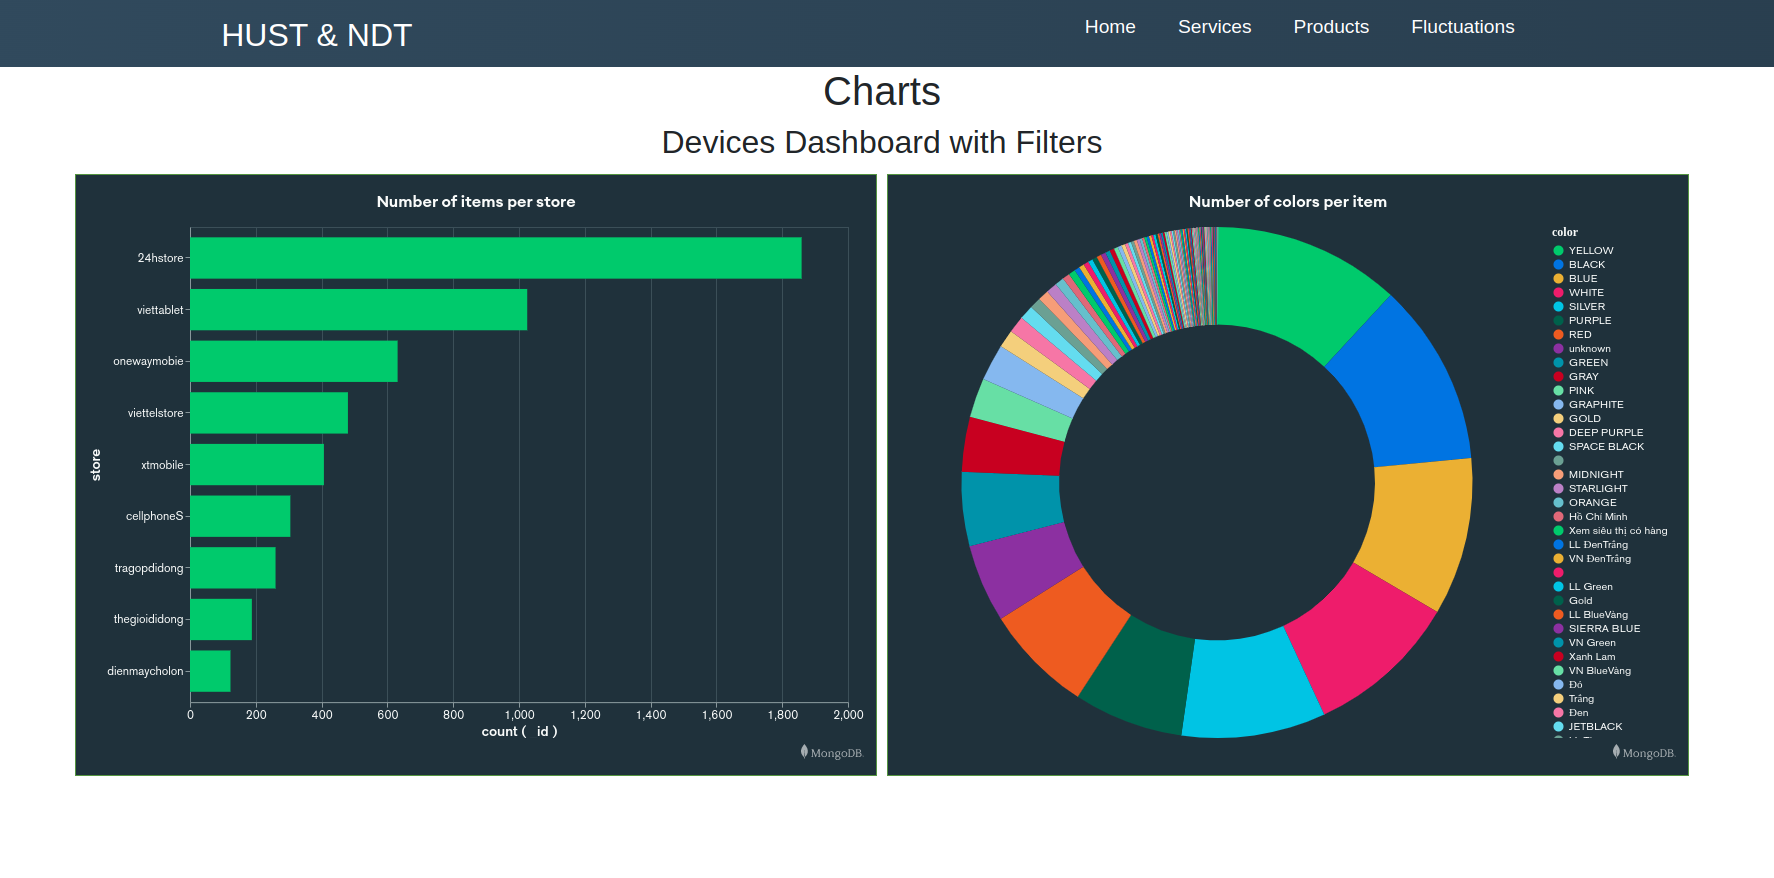
\includegraphics[scale=0.25]{Hinhve/chart_UI.png}
    \caption{Màn hình xem biểu đồ}
    \label{fig:my_label2}
\end{figure}

Bên cạnh đó người quản trị có thể tùy chỉnh hoặc xây dựng các dashboard để theo dõi những số liệu biểu đồ nhằm phân tích cũng như đưa ra nhận định xu hướng đúng đắn của thị trường. Mongodb cloud hỗ trợ tính năng xây dựng dashboard đơn giản nhanh chóng truy vấn dữ liệu trực tiếp từ cơ sở dữ liệu từ đó hiển thị với tốc độ nhanh, được làm mới liên tục.
Sau đây là một vài phân tích cơ bản của các biểu đồ 


\begin{figure}[H]
    \centering
    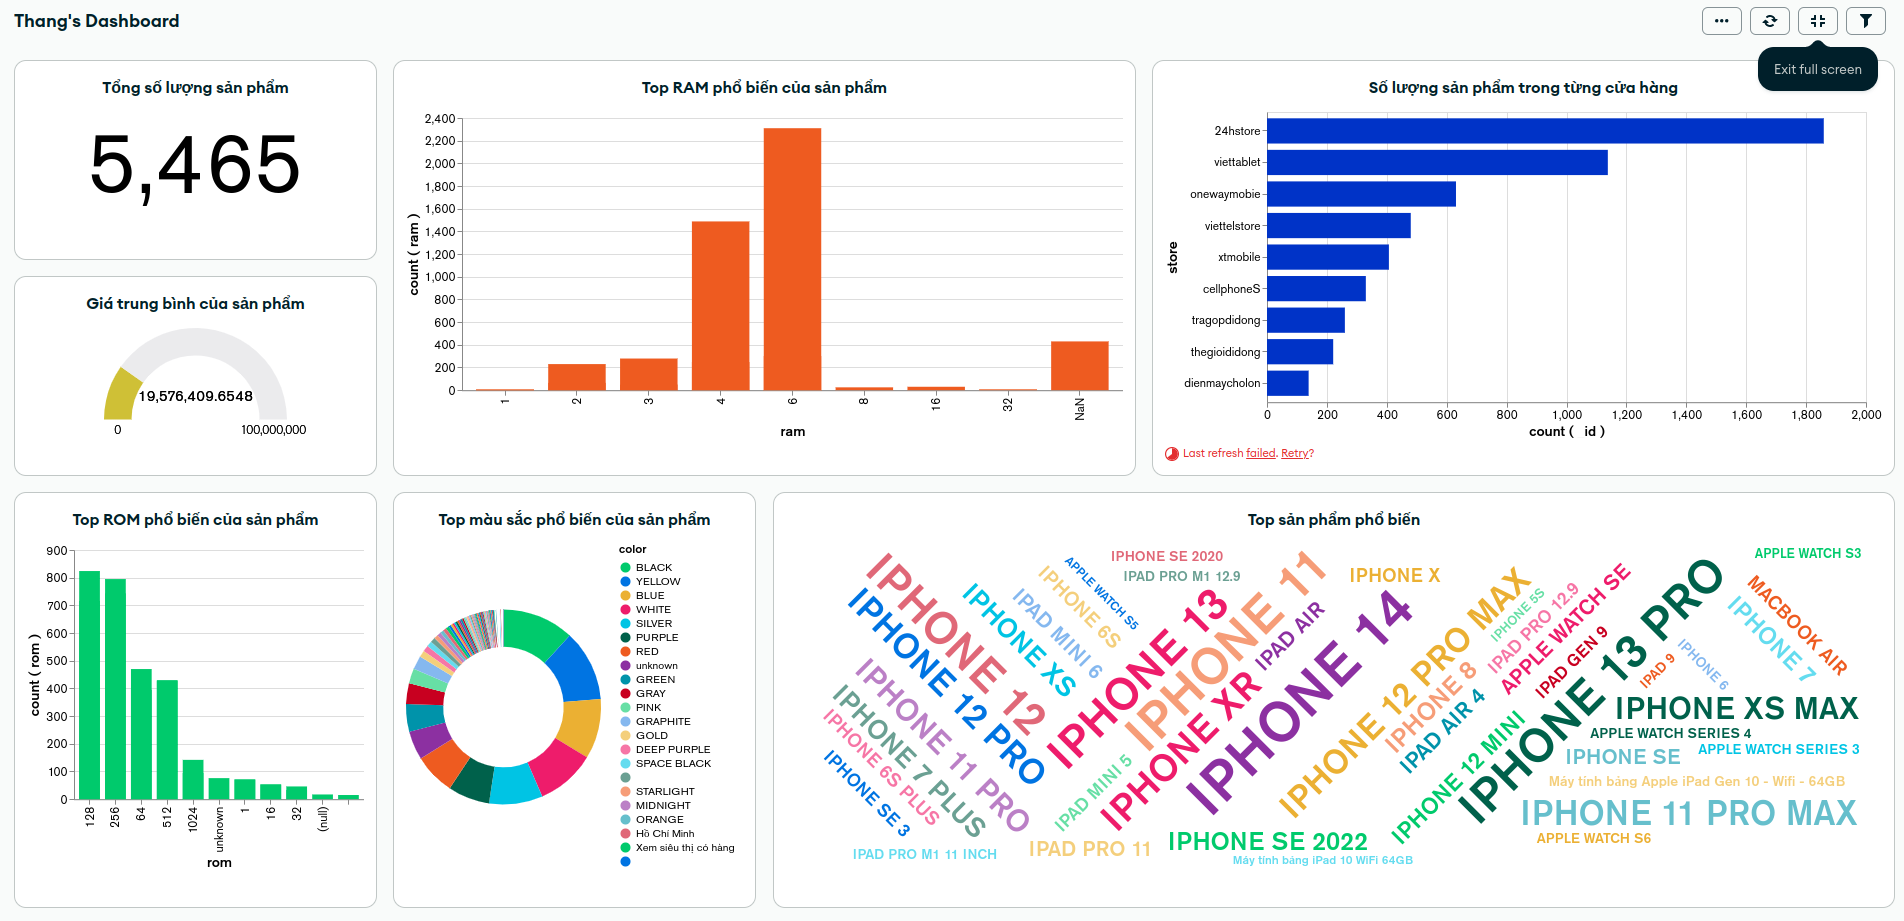
\includegraphics[scale=0.22]{Hinhve/dashboard.png}
    \caption{Dashboard}
    \label{fig:my_label2}
\end{figure}

\begin{figure}[H]
    \centering
    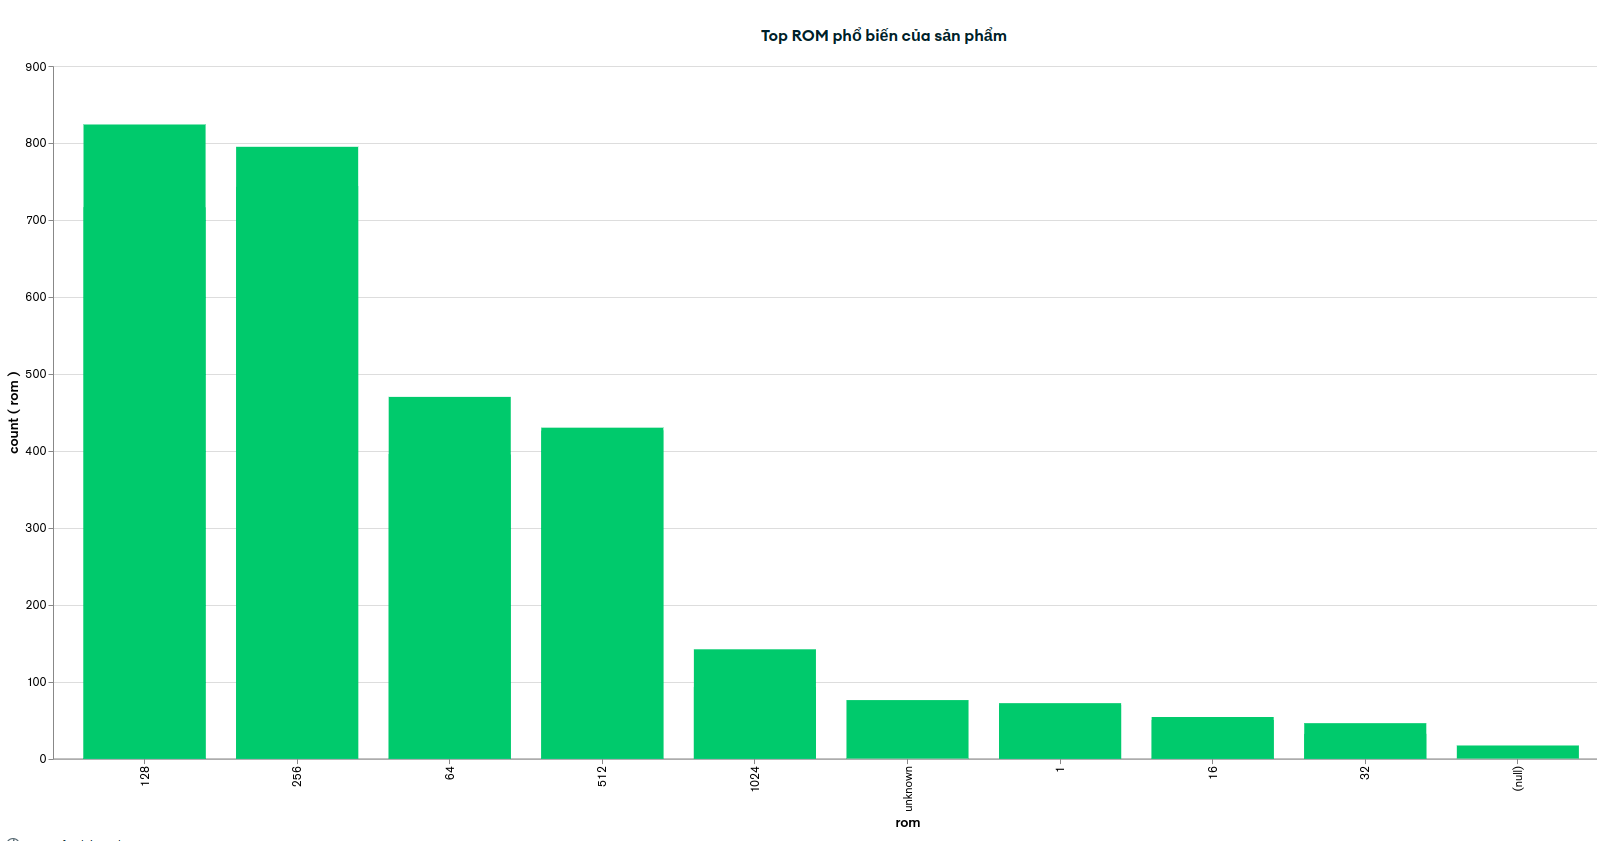
\includegraphics[scale=0.25]{Hinhve/topRom.png}
    \caption{Top rom phổ biến}
    \label{fig:my_label2}
\end{figure}

\begin{figure}[H]
    \centering
    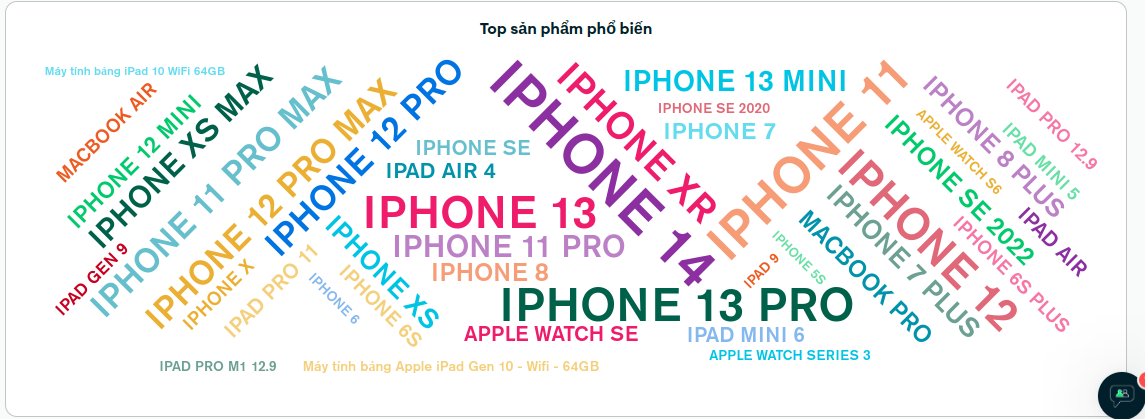
\includegraphics[scale=0.4]{Hinhve/topProduct.png}
    \caption{Top sản phẩm phổ biến}
    \label{fig:my_label2}
\end{figure}

\begin{figure}[H]
    \centering
    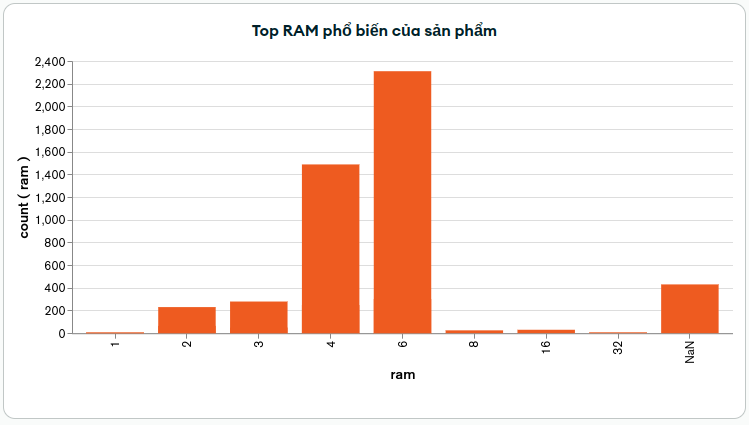
\includegraphics[scale=0.55]{Hinhve/topRam.png}
    \caption{Top ram phổ biến}
    \label{fig:my_label2}
\end{figure}

\begin{figure}[H]
    \centering
    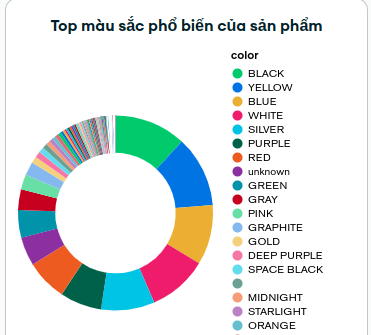
\includegraphics[scale=0.7]{Hinhve/topColor.png}
    \caption{Top màu sắc phổ biến}
    \label{fig:my_label2}
\end{figure}

\begin{figure}[H]
    \centering
    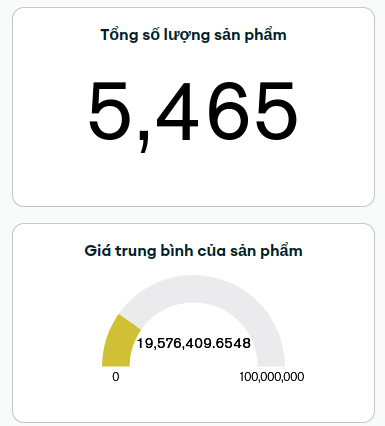
\includegraphics[scale=0.8]{Hinhve/topNumber.png}
    \caption{Thống kê}
    \label{fig:my_label2}
\end{figure}

Chương này đã mô tả chi tiết về hệ thống tích hợp dữ liệu từ việc thu thập, xử lý đến việc lưu trữ và ứng dụng vào tìm kiếm sản phẩm cho người dùng. Hệ thống đảm bảo luồng dữ liệu được thống nhất và tạo thành một đường ống dữ liệu xuyên suốt hệ thống cập nhật hàng ngày, hàng giờ tùy vào nhu cầu của người dùng. Tuy nhiên trong quá trình thiết kế và xây dựng hệ thống có gặp phải những vấn đề khó khăn và thách thức đòi hỏi những giải pháp thay thế, những cách làm khác đáp ứng yêu  và cải thiện hiệu năng của hệ thống. Vấn đề này sẽ được trình bày ở phần tiếp theo của quyển đồ án.
\end{document}
